

\section{Algoritmos de aprendizaje profundo y TensorFlow}
\subsection{Aprendizaje automático}\label{aprendizaje-automuxe1tico}

\begin{remark}
Un algoritmo de
aprendizaje automático es un algoritmo que tiene la capacidad de
aprender a partir de datos.
\end{remark}

\begin{remark}
Un programa de computadora se dice que aprende de la experiencia $E$ con
respecto a alguna clase de tarea $T$ y una medida de desempeño $P$, si su
desempeño de tareas en $T$, medido por $P$, mejora con la experiencia $E$.
\end{remark}


\subsubsection{La tarea T}\label{la-tarea-t}

Las tareas son difíciles de resolver con programas estáticos escritos y
diseñados por humanos.
Aprender es el medio para tener la habilidad de realizar una tarea.

Las tareas del aprendizaje automático son descritas en términos de cómo
el sistema de aprendizaje automático debe procesar una muestra.\\

\begin{remark}
Una muestra es una colección de características que han sido medidas
cuantitativamente a partir de un objeto o evento que queremos que
nuestro sistema de aprendizaje automático procese. De manera típica una
muestra se representa como un vector $\mathbf{x} \in \mathbb{R}^{n}$ donde cada elemento
$x_i$ del vector es una característica.
\end{remark}

Muchos tipos de tareas se pueden resolver con aprendizaje automático.
Algunas de las tareas más comunes en el aprendizaje automático incluyen
las siguientes:

\begin{itemize}
    \item \textbf{Clasificación}: En este tipo de tarea, se le pregunta al programa a cuál
    de $k$ categorías pertenece una entrada. Para resolver esta tarea, el
    algoritmo de aprendizaje generalmente produce una
    función $f : \mathbb{R}^n \rightarrow \{1, \dots, k\}$. Cuando $y = f(\mathbf{x})$, el
    modelo asigna una entrada descrita por el vector $\mathbf{x}$ a una categoría
    identificada por un código numérico $y$.
    \item \textbf{Clasificación con entradas faltantes}: La clasificación se vuelve más difícil si al programa no se le garantiza que cada medida en su vector de entradas,
    será dada siempre. Para resolver la tarea de clasificación, el
    algoritmo de aprendizaje sólo tiene que definir una función que mapee de
    un vector de entradas a una salida categórica. Cuando algunas entradas
    faltan, más que proveer una sola función de clasificación, el algoritmo
    de aprendizaje debe aprender de un conjunto de funciones. Cada función
    corresponde a clasificar $\mathbf{x}$ con un subconjunto diferente de entradas
    faltantes. Una manera eficiente de definir un conjunto
    tan grande de funciones es aprender la distribución de probabilidad
    sobre todas las variables relevantes, entonces resolver la tarea de
    clasificación marginalizando las variables faltantes. Con $n$ variables de
    entrada, podemos obtener todas las $2^n$ funciones de clasificación que
    se necesitan para cada conjunto de entradas faltantes posible, pero sólo
    se necesita aprender una función que describa la distribución de
    probabilidad conjunta.
    \item \textbf{Regresión}: En este tipo de tarea, al programa se le solicita predecir un valor numérico dada una entrada.
    Para resolver esta tarea, al algoritmo de aprendizaje se le pide que
    genere una función $f: \mathbb{R}^n \rightarrow \mathbb{R}$. Este tipo de tarea es
    similar al de clasificación, excepto que el formato de la salida es
    diferente. 
    \item \textbf{Transcripción}: En este tipo de
    tarea, al sistema de aprendizaje automático se le pide observar la
    representación relativamente no estructurada de algún tipo de
    información y transcribirlo de una forma textual y discreta.
    \item \textbf{Traducción máquina}: En una tarea de traducción
    máquina, la entrada consiste de una secuencia de símbolos en algún
    lenguaje, y el programa de computadora debe convertir esto en una
    secuencia de símbolos en otro lenguaje.
    \item \textbf{Salida estructurada}: Las tareas de salida estructurada involucran cualquier
    tarea donde la salida es un vector (o cualquier otro tipo de estructura
    de datos que contenga múltiples valores) con relaciones importantes
    entre los diferentes elementos. Esta categoría subsume las tareas
    como la traducción y transcripción. Estas tareas son
    llamadas así porque el programa debe producir varios valores que están
    estrechamente interrelacionados.
    \item  \textbf{Detección de anomalías}: En este tipo de
    tarea, el programa examina cuidadosamente un conjunto de eventos u
    objetos, y marca algunos de ellos por ser atípicos o inusuales.
    \item \textbf{Síntesis y muestreo}
    (sampling): En este tipo de tarea se le solicita al algoritmo de
    aprendizaje automático que genere nuevas muestras que son similares a
    las de un conjunto de entrenamiento. La síntesis y muestreo a través de
    aprendizaje automático, puede ser útil en aplicaciones multimedia donde
    puede ser caro o cansado para un artista generar grandes volúmenes de
    contenido a mano. En algunos casos, se
    quiere que el procedimiento de muestreo y síntesis genere algún tipo de
    salida específica dada la entrada.
    \item \textbf{Atribución de valores faltantes}: En este tipo de tarea, al algoritmo de
    aprendizaje máquina se le da una nueva muestra $\mathbf{x} \in \mathbb{R}^n$, pero con
    algunos elementos $x_i$ de $\mathbf{x}$ faltantes. El algoritmo debe predecir los
    valores de las entradas faltantes. 
    \item \textbf{Reducción de ruido}: En este tipo de
    tarea, el algoritmo de aprendizaje automático recibe como una entrada
    una muestra corrupta $\mathbf{x}' \in \mathbb{R}^n$, obtenido por un proceso de corrupción
    desconocido de una muestra limpia $\mathbf{x} \in \mathbb{R}^n$. El aprendiz debe predecir la
    muestra limpia $\mathbf{x}$ de su versión corrupta $\mathbf{x}'$ , o de manera más general
    predecir la distribución de probabilidad condicional $P(\mathbf{x} | \mathbf{x}')$.


\end{itemize}
    


\subsubsection{La medida de desempeño
P}\label{la-medida-de-desempeuxf1o-p}

A fin de que se puedan evaluar las habilidades de un algoritmo de
aprendizaje automático, se debe diseñar una medida cuantitativa de su
desempeño. Usualmente esta medida de desempeño $P$ es específica a la
tarea $T$ que se lleva a cabo por el sistema.

Para tareas de clasificación, clasificación con entradas faltantes, y
transcripción, se mide la precisión (\textit{accuracy}) del modelo. \\

\begin{remark}
La precisión
es sólo la proporción de muestras para los cuales el modelo produce la
salida correcta. Se puede obtener una información equivalente midiendo
la tasa de error, la proporción de muestras para las cuales el modelo
produce la salida incorrecta.
\end{remark}

% Con frecuencia nos referimos a la tasa de
% error como la pérdida $0-1$. La pérdida $0-1$ sobre una muestra en
% particular es $0$ si está clasificada correctamente y $1$ si no.

Usualmente estamos interesados en cómo se desempeña un algoritmo de
aprendizaje automático sobre datos que no ha visto,
ya que determina que tan bien trabajará cuando se lance al mundo real.
Por lo tanto evaluamos estas medidas de desempeño usando un \textit{conjunto de
prueba}, que está separado de los datos usados para entrenar el sistema
de aprendizaje automático.

\subsubsection{La experiencia E}

Los algoritmos de aprendizaje automático pueden ser de manera muy
general categorizados como \textit{supervisados} o \textit{no supervisados} por el tipo de
experiencia que tienen disponible durante el proceso de aprendizaje.

A la mayoría de los algoritmos de aprendizaje se les permite
experimentar un \textit{conjunto de datos}.\\

\begin{remark}
Un conjunto de datos es un
colección de muchas muestras. Algunas veces a esas muestras se les llama
\textit{patrones de entrada}.
De manera muy general un conjunto de datos
es una colección de muestras, que a su vez son colecciones de \textit{características}.
\end{remark}


\subsubsection{Algoritmos de aprendizaje no supervisados}

\begin{remark}
Los algoritmos de aprendizaje no supervisados experimentan un conjunto
de datos que contiene una gran cantidad de características, entonces aprenden algunas
propiedades útiles de la estructura del conjunto de datos. 
\end{remark}

Algunos algoritmos no supervisados realizan papeles como el 
de agrupamiento, que consiste en dividir el conjunto de 
datos en grupos de muestras similares.\\


\begin{remark}
El aprendizaje no supervisado involucra observar
varias muestras de un vector aleatorio $\mathbf{x}$, e intentar aprender implícita
o explícitamente la distribución de probabilidad $P(\mathbf{x})$, de algunas
propiedades interesantes de la distribución.
\end{remark}


\subsubsection{Algoritmos de aprendizaje
supervisados}

\begin{remark}
Los algoritmos de aprendizaje supervisados experimentan un conjunto de
datos que contiene características, pero cada muestra está asociada además con
una \textit{etiqueta} u \textit{objetivo}.
El aprendizaje supervisado involucra observar bastantes muestras de un
vector aleatorio $\mathbf{x}$ y un valor o vector asociado $\mathbf{y}$, y aprender a
predecir $\mathbf{y}$ a partir de $\mathbf{x}$, usualmente estimando $P(\mathbf{y} |\mathbf{x})$.
\end{remark}



\subsubsection{Capacidad, sobreajuste e
infra-ajuste}

El principal reto del aprendizaje automático es que se debe desempeñar
bien sobre entradas nuevas no vistas previamente, no sólo con las que el
modelo fue entrenado. La habilidad de desempeñarse bien sobre entradas
no observadas previamente se llama \textit{generalización}.

Comúnmente cuando se entrena un modelo de aprendizaje automático, se
tiene acceso a un \textit{conjunto de entrenamiento}, se puede calcular alguna
medida de error sobre el conjunto de entrenamiento llamado error de
entrenamiento, y reducir este error. Hasta acá, simplemente se ha descrito
un problema de optimización ya que se pretende encontrar la mejor solución.
Lo que distingue al aprendizaje automático de la optimización es que
queremos que el \textit{error de generalización}, también llamado error de
prueba, sea bajo también.\\

\begin{remark}
El error de generalización se define como el valor esperado del error de
una nueva entrada. Aquí la esperanza es tomada a través de diferentes
entradas posibles. extraída de la distribución de entradas que esperamos
el sistema se encuentre en la práctica.
\end{remark}


Típicamente estimamos el error de generalización de un modelo de
aprendizaje automático midiendo su desempeño sobre un conjunto de prueba de
muestras que fueron recolectadas de manera separada del conjunto de
entrenamiento.

¿Cómo se puede afectar el desempeño sobre el conjunto de pruebas cuando
sólo se ha observado el conjunto de entrenamiento? 
% El campo de la
% \textit{teoría del aprendizaje estadístico} provee varias respuestas.
% Si el conjunto de entrenamiento y el de prueba son recolectados de manera
% arbitraria, entonces no se puede hacer mucho. Si podemos hacer
% algunas suposiciones sobre cómo el conjunto de prueba y de entrenamiento
% se ``recogen'', entonces podemos hacer algún progreso.
Mediante un \textit{proceso de generación de datos} los conjuntos de 
entrenamiento y de prueba son producidos por una 
distribución de probabilidad sobre conjuntos de datos. 
Se hacen un conjunto de suposiciones conocidas
colectivamente como las suposiciones i.i.d. Estas suposiciones son que
las muestras en cada conjunto de datos son independientes entre sí, y
los conjuntos de entrenamiento y de prueba están idénticamente
distribuidos. Esta suposición nos permite describir el proceso de
generación de datos con una distribución de probabilidad sobre una sola
muestra. La misma distribución es usada para generar cada muestra de
entrenamiento y cada muestra de prueba. Llamamos a la distribución
mencionada la distribución de generación de datos, denotada por $p_{data}$.
Este marco de trabajo probabilístico y las suposiciones i.i.d. permiten
estudiar matemáticamente la relación entre el error de entrenamiento y
el error de prueba.

Se puede observar que el valor esperado del error de entrenamiento de un
modelo seleccionado aleatoriamente es igual al valor esperado del error
de prueba del modelo. Supongamos que tenemos una distribución de
probabilidad $P(x, y)$ y obtenemos muestras de esta repetidamente para
generar el conjunto de entrenamiento y el conjunto de prueba. Para algún
valor fijo $w$, el valor esperado del error de entrenamiento es
exactamente el mismo que el valor esperado del conjunto de prueba,
porque ambas esperanzas están formadas usando el mismo proceso de
muestreo. La única diferencia entre las dos condiciones es el nombre que
asignamos al conjunto de datos que muestreamos.

Cuando usamos un algoritmo de aprendizaje automático, no
se fijan los parámetros antes de tiempo y luego se hace el muestreo de
los conjuntos de datos. Muestreamos el conjunto de entrenamiento,
entonces se eligen los parámetros para reducir el error de
entrenamiento, luego se hace el muestreo del conjunto de prueba. Los
factores que determinan que tan bien se desempeña un algoritmo de
aprendizaje automático son la habilidad de:

\begin{itemize}
    \item Minimizar el error de entrenamiento.
    \item Minimizar la diferencia entre el error de entrenamiento y el de prueba.
\end{itemize}



Estos dos factores corresponden a los dos retos principales en el
aprendizaje automático: \textit{sobreajuste} e \textit{infra-ajuste}.\\ 

\begin{remark}
El infra-ajuste
ocurre cuando el modelo no puede obtener un valor en el error lo
suficientemente bajo sobre el conjunto de entrenamiento. El sobreajuste
ocurre cuando la diferencia entre el error de entrenamiento y de prueba
es muy grande.
\end{remark}


Se puede controlar cuando un modelo es más propenso a sobre ajustarse o
infra-ajustarse alterando su capacidad.\\

\begin{remark}
La capacidad de un
modelo es la habilidad de ajustarse a una amplia variedad de funciones.
Modelos con baja capacidad pueden esforzarse por ajustarse a su conjunto
de entrenamiento. Los modelos con alta capacidad pueden sobre ajustarse
memorizando propiedades del conjunto de entrenamiento que no pueden
funcionar bien sobre el conjunto de prueba.
\end{remark}


Una manera de controlar la capacidad de un algoritmo de aprendizaje es
eligiendo un conjunto de hipótesis, el conjunto de funciones de donde el
algoritmo de aprendizaje puede seleccionar la solución. 
Los algoritmos de aprendizaje automático generalmente se desempeñarán
mejor cuando su capacidad es apropiada en lo que respecta a la verdadera
complejidad de la tarea que necesitan realizar y la cantidad de datos de
entrenamiento que utilizan. Modelos con capacidad insuficiente son
incapaces de resolver tareas complejas. Modelos con alta capacidad
pueden resolver tareas complejas, pero cuando su capacidad es mayor de
la necesaria para resolver la tarea, tienden a sobre ajustarse.

La capacidad no está determinada únicamente por la elección del modelo.
El modelo especifica qué familia de funciones el algoritmo de
aprendizaje puede elegir donde se varían los parámetros para reducir el
objetivo de entrenamiento. Esa es llamada la \textit{capacidad representacional}
del modelo. En muchos casos, la mejor función dentro de esa familia de
funciones es un problema de optimización muy difícil. En la práctica, el
algoritmo de aprendizaje no encuentra la mejor función, pero sí una que
reduce el error de entrenamiento significativamente. Estas limitantes
adicionales como la imperfección del algoritmo de optimización,
significan que la capacidad efectiva puede ser menor que la capacidad
representacional de la familia del modelo.


\subsubsection{Optimización basada en el gradiente}

La mayoría de los algoritmos de aprendizaje involucran la optimización 
de alguna forma. La optimización se refiere a la tarea de ya sea 
minimizar o maximizar una función $f(\mathbf{x})$ alterando $\mathbf{x}$.

La función que queremos minimizar o maximizar se conoce como \textit{función objetivo}.
En el contexto del aprendizaje automático, queremos minimizar una \textit{función
de costo} que mide el error de entrenamiento. 

Antes de avanzar conviene repasar algunos conceptos de cálculo
relacionados con la optimización.
Supongamos que tenemos la función $y = f(x)$, donde $x$ y $y$ son números reales.
La \textit{derivada} de la función se denota como $f'(x)$ o $\frac{dy}{dx}$.
La derivada $f'(x)$ da la pendiente de la recta tangente de $f(x)$ en el punto x.
La derivada
especifica como se puede escalar un cambio menor en la entrada de manera que se obtenga
el cambio correspondiente en la salida: $f(x + \gamma) \approx f(x) + \gamma f'(x)$.

La derivada por lo tanto es útil para minimizar una función porque nos dice
cómo cambiar $x$ para hacer un decremento en $y$. Por ejemplo, sabemos que
$f(x - \gamma  \text{ sgn} (f'(x)))$ es menor que $f(x)$ para un $\gamma$ lo
suficientemente menor. Podemos reducir $f(x)$ moviendo $x$ en pequeños pasos
con el signo opuesto a la derivada. Esta técnica se llama \textit{descenso del gradiente}.

\begin{figure}[ht]
    \centering
    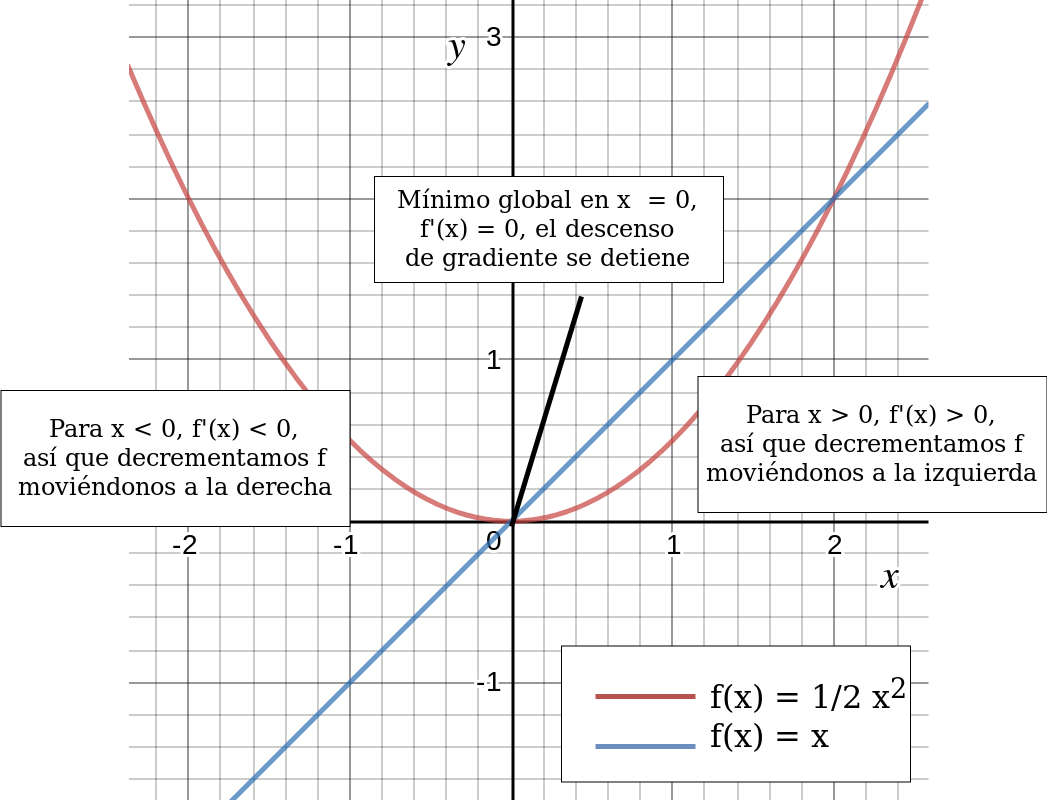
\includegraphics[scale=0.2]{gradient_descent.png}
    \caption{El método del descenso del gradiente utiliza las derivadas de una función para ir cuesta abajo hasta llegar a un mínimo.}
    \label{fig:gradient_descent_first_example}
\end{figure}

Cuando $f'(x) = 0$ la derivada no provee ninguna información sobre la dirección
en la cual moverse. Puntos donde $f'(x) = 0$ se conocen como 
\textit{puntos críticos}. Un \textit{mínimo local} es un punto donde $f(x)$ es
menor que todos sus puntos vecinos, así que no es posible 
disminuir $f(x)$ haciendo pasos infinitesimales. Un \textit{máximo local} es
un punto donde $f(x)$ es mayor que todos los puntos vecinos, así que no es posible
incrementar $f(x)$ con pasos infinitesimales. Algunos puntos críticos no son
ni máximos ni mínimos, son llamados \textit{puntos de silla}.

Un punto que obtiene el valor menor absoluto de $f(x)$ es un \textit{mínimo global}.
Es posible que un mínimo local no sea globalmente óptimo. En el contexto
del aprendizaje profundo, se optimizan funciones que 
pueden tener mínimos locales que no son óptimos, y puntos de silla 
atrapados por regiones planas. Esto hace el proceso de optimización
muy complicado, especialmente si la función es multidimensional.
Por esto, usualmente se busca un valor de $f$ muy bajo, pero
no necesariamente el mínimo en un sentido formal.

Comúnmente se minimizan funciones que tienen múltiples entradas 
$f: \mathbb{R}^n \rightarrow \mathbb{R}$. Para funciones con varias entradas,
se hace uso del concepto de \textit{derivada parcial}. La derivada
parcial $\frac{\partial f(\mathbf{x})}{\partial x_i} $ mide cómo
cambia $f$ cuando sólo la variable $x_i$ se incrementa en el punto $\mathbf{x}$.\\

\begin{remark}
El \textit{gradiente} generaliza la noción de derivada para el caso
donde la derivada es con respecto a un vector: el gradiente de $f$ es el
vector que contiene todas las derivadas parciales, denotado por $\nabla f(\mathbf{x})$. El i-ésimo elemento del gradiente es la 
derivada parcial de $f$ con respecto a $x_i$. En múltiples dimensiones,
los puntos críticos son puntos donde cada elemento del gradiente es igual 
a cero.
\end{remark}

\begin{remark}
La \textit{derivada direccional} mide  la tasa de cambio de una función
en un punto sobre un vector. 
La derivada direccional en la dirección $\mathbf{u}$ (un vector
unitario) es la pendiente de la función $f$ en la dirección $\mathbf{u}$ y se denota como $D_\mathbf{u}f(\mathbf{x})$.
\end{remark}

Para minimizar $f$, nos gustaría encontrar la dirección en la que $f$ disminuye
más rápidamente. Esto se puede hacer a través de la derivada direccional.

\[
\begin{array}{rcl}
            D_\mathbf{u}f(\mathbf{x}) & = & \nabla f(\mathbf{x}) \cdot \mathbf{u}\\
           & = & \|\nabla f(\mathbf{x})\| \|\mathbf{u}\| \cos({\theta})\\
           & = & \|\nabla f(\mathbf{x})\| \cos({\theta})
   \end{array}
\]

se puede ver que el valor máximo de $D_\mathbf{u}f(\mathbf{x})$
se alcanza cuando $\cos({\theta}) = 1$. Por lo tanto $\theta = 0$, y
el valor máximo de la derivada direccional se tiene cuando $\mathbf{u}$
tiene la misma dirección que $\|\nabla f(\mathbf{x})\|$. Este valor
máximo de $D_\mathbf{u}f(\mathbf{x})$ es

\[
\|\nabla f(\mathbf{x})\| \cos({\theta}) = \|\nabla f(\mathbf{x})\| 
\]

De igual forma, el valor mínimo de $D_{\mathbf{u}f(\mathbf{x})}$ puede obtenerse haciendo $\theta  = \pi$ de manera que 
$\mathbf{u}$ apunte a la dirección opuesta de $\nabla f(\mathbf{x})$.\\


\begin{remark}
La derivada direccional $D_\mathbf{u}f(\mathbf{x})$ tiene un valor
máximo $\|\nabla f (\mathbf{\mathbf{x}})\|$
cuando $\mathbf{u}$ tiene la misma dirección que $ \nabla f (\mathbf{x})$ y un mínimo valor $-\|\nabla f (\mathbf{\mathbf{x}})\|$ cuando $\mathbf{u}$ tiene la dirección que $-\nabla f (\mathbf{\mathbf{x}})$. En otras palabras, el vector
gradiente apunta en la dirección de la máxima tasa de crecimiento de la función
y el vector gradiente negativo apunta a la máxima tasa de disminución de la 
función.
\end{remark}

\begin{remark}
Podemos disminuir $f$
moviéndonos en la dirección del gradiente negativo. Esto es conocido
como \textit{el método del descenso más empinado} o \textit{descenso del gradiente}.

El descenso del gradiente propone un nuevo punto

\[
\mathbf{x}' = \mathbf{x} - \gamma \nabla f(\mathbf{x})
\]


donde $\gamma$ es la \textit{tasa de aprendizaje}, un escalar positivo
que determina el tamaño de los pasos. Se puede elegir $\gamma$
de diferentes maneras, pero es muy común que $\gamma$
se defina como una constante pequeña.
\end{remark}

El descenso del gradiente converge cuando cada elemento del gradiente es 
cero (en la práctica son valores muy cercanos a cero).

Resumiendo, la manera en la que el método del descenso del gradiente
trabaja, es calculando repetidamente el gradiente $\nabla f(\mathbf{x})$,
y después se moviéndose en la dirección opuesta. Con esto se disminuirá $f$ hasta 
posiblemente alcanzar un mínimo global.

\subsubsection{Terminología}

A continuación se definen diferentes términos que se utilizan a lo
largo del trabajo.

\begin{itemize}

\item
  \textbf{Ejemplos o muestras}: objetos o instancias de información usadas para
  aprender o evaluar.
 \item
 \textbf{Características}: El conjunto de atributos, comúnmente representadas
como un vector, asociado a una muestra. 
\item 
\textbf{Etiquetas}: Valores o categorías
asignadas a muestras. 
\item \textbf{Muestra de entrenamiento}: Las muestras usadas
para entrenar un algoritmo. 
\item 
\textbf{Muestra de validación}: Muestras usadas
para ajustar los parámetros de un algoritmo de aprendizaje cuando se
trabaja con datos etiquetados. Los algoritmos de aprendizaje usualmente
tienen uno o más parámetros libres, y la muestra de validación es usada
para seleccionar los valores apropiados para los parámetros del modelo.
\item 
\textbf{Muestra de prueba}: Muestras usadas para evaluar el desempeño de un
algoritmo de aprendizaje. La muestra de prueba está separada del
conjunto de entrenamiento y validación, y no está disponible en la etapa
de aprendizaje. 
\item
\textbf{Función de costo}: También llamada función de error o de pérdida. 
Es una función que mide la
diferencia, o pérdida, entre la etiqueta predicha y la verdadera.
Denotando al conjunto de todas las etiquetas como $Y$ y al conjunto de
todas las posibles predicciones como $Y'$, una función $C$ es una mapeo $C: Y
 \times Y' \rightarrow \mathbb{R}^+$. En la mayoría de los casos $Y = Y'$ y la función
de pérdida está acotada, pero estas condiciones no se cumplen siempre.
Algunos ejemplos comunes de funciones de pérdida incluyen la $0-1$,
definida como $C(y, y') = 1$ si $y \neq y'$ y la pérdida cuadrada definida por
$C(y, y') = (y' - y)^2$. 
\item
\textbf{Conjunto de hipótesis}: Un conjunto de
funciones que mapean características (vectores de características) al
conjunto de etiquetas $Y$. De manera más general, las hipótesis pueden ser
funciones que mapean las características a un conjunto diferente $Y'$.
\end{itemize}



\subsection{Redes neuronales artificiales}


En su forma más general, una \textit{red neuronal artificial} 
o simplemente \textit{red neuronal}, es una máquina diseñada para modelar la manera en la cual el cerebro 
realiza una tarea en particular o una función de interés. Las redes neuronales 
artificiales utilizan
una enorme cantidad de interconexiones de células de cómputo conocidas como neuronas o unidades de procesamiento.\\


\begin{remark}
Una red neuronal artificial es un procesador paralelo distribuido construido de unidades simples de
procesamiento, que tiene una naturaleza propensa a almacenar
conocimiento basado en experiencias y poniéndolo a disposición para su uso. Se 
asemeja al cerebro en dos aspectos:
\begin{enumerate}
    \item El conocimiento es adquirido por la red desde su ambiente a través de un proceso de aprendizaje. El proceso de aprendizaje se hace a través de un algoritmo de aprendizaje.
    \item Las fuerza de conexión entre neuronas, también conocidas como pesos sinápticos, son usadas para almacenar el conocimiento adquirido.
\end{enumerate}

\end{remark}

En términos generales, una red neuronal artificial consiste un de un gran número 
de procesadores simples enlazados por conexiones ponderadas.
Cada unidad recibe entradas que vienen de muchas otras unidades y 
produce un valor escalar como salida que depende sólo de la información
disponible localmente, ya sea de la que guarda internamente o la que llega
a través de las conexiones ponderadas. La información es distribuida 
y actúa como entrada a otras unidades de procesamiento.

Por sí mismo, un elemento de procesamiento no es muy poderoso; el poder
del sistema surge de la combinación de muchas unidades en una red.
Una red está especializada en implementar diferentes funciones cambiando la 
topología de las conexiones en la red y los valores de las
conexiones ponderadas.

Las unidades de procesamiento tienen respuestas como

\begin{equation}\label{eq:neuron-output}
y = f\bigg (\sum_k w_k x_k\bigg )    
\end{equation}

donde $x_k$ son las señales de salida de otros nodos o entradas de un sistema
externo, $w_k$ son los pesos de los enlaces de conexión y $f$ es una función
no lineal. Aquí una la unidad calcula una combinación lineal de los pesos y sus
entradas y la pasa por $f$ para producir un valor escalar. 
$f$ es conocida como \textit{función de activación}, y es muy común que
se utilice una función no lineal acotada y creciente como la sigmoide, definida como sigue

\[
f(u) = \frac{1}{1 + e^{-u}}
\]

\begin{figure}
    \centering
    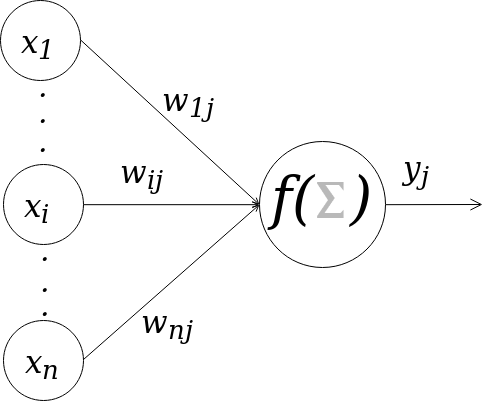
\includegraphics[scale=0.30]{neuron.png}
    \caption{Un modelo de una neurona, la unidad más simple de procesamiento en la red.}
    \label{fig:neuron}
\end{figure}
El término perceptrón a menudo se utiliza para referirse a cualquier
red de nodos \textit{feedforward} con respuestas como la ecuación (\ref{eq:neuron-output}).
Una red puede tener cualquier estructura arbitraria, sin embargo, 
las arquitecturas en capas son muy populares.\\

\begin{remark}
El perceptrón
multicapa o MLP (por sus siglas en inglés), es ampliamente utilizado.
En tales estructuras las unidades en la capa $L$ reciben entradas de la capa
que les precede $L-1$ y envía sus salidas a la capa siguiente $L+1$. Entradas
externas se presentan en la primera capa y las salidas del sistema se toman
de la última capa. Las capas internas se llaman \textit{capas ocultas}. Las redes
más simples tienen una sola capa activa, las de las unidades de salida, por convención, las entradas no se cuentan como una capa activa ya que no realizan
algún tipo de procesamiento. Las redes con una sola capa son menos 
poderosas que las multicapas por lo que sus aplicaciones están
muy limitadas.
\end{remark}

\begin{figure}
    \centering
    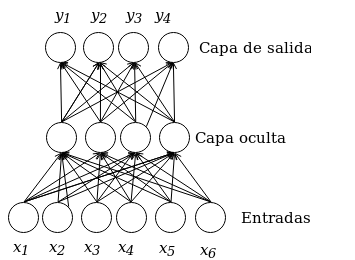
\includegraphics[scale=0.5]{mlp.png}
    \caption{Una red neuronal feedforward completamente conectada con múltiples capas.}
    \label{fig:mpl}
\end{figure}

Que una estructura sea \textit{feedforward} o \textit{prealimentada} significa 
que no existen bucles en la red, la información siempre alimenta
hacia adelante, nunca hacia atrás. La red implementa un
mapeo estático que depende únicamente de las entradas que se presenten y es 
independiente de los estados previos del sistema.\\

\begin{remark}
En una red \textit{completamente conectada}, cada nodo en la capa $L$
recibe entradas de cada nodo en la capa anterior $L-1$ y envía su salida
a todos los nodos en la capa $L+1$.
\end{remark}

Las redes neuronales pueden verse como
gráficas cuyos nodos son unidades de cálculo y cuyas aristas
transmiten información numérica de nodo a nodo. Cada unidad de cómputo es capaz de evaluar su entrada
en una función de activación. La red representa una cadena de funciones compuestas,
que transforman una entrada en un vector de salida. La red es una implementación
particular de una función compuesta desde la entrada hasta el espacio de salida,
a la cual llamamos \textit{función de red}.

En el contexto del aprendizaje automático supervisado,
la experiencia de la que aprenden las redes neuronales es un conjunto 
con patrones de entrada donde cada patrón tiene una salida deseada.
Nuestro problema de aprendizaje consiste
en encontrar la combinación de pesos óptima tal que la función de red 
$\varphi$ se aproxime lo más que se pueda a una función $F$. Sin embargo,
no contamos con la función $F$ explícitamente, sino sólo a través de algunas muestras.

Consideremos una red prealimentada 
con $n$ unidades de entrada y $m$
unidades de salida. Ésta consiste de cualquier número de unidades ocultas
y de cualquier topología en sus conexiones. También contamos
con un conjunto de entrenamiento 
$\{(\mathbf{x}_1, \mathbf{t}_1), \dots, (\mathbf{x}_p, \mathbf{t}_p)\}$, con $p$ pares ordenados de vectores de tamaño $n$ y $m$, los cuales se llaman patrones de entrada y de salida.
Definamos a las funciones de activación de cada nodo en la red como
continuas y diferenciables. Los pesos de las aristas son números reales 
seleccionados aleatoriamente. Cuando el patrón de entrada $\mathbf{x}_i$
del conjunto de entrenamiento se presenta en la red, produce una salida 
$\mathbf{y}_i$, generalmente diferente al objetivo $\mathbf{t}_i$.
Queremos que $\mathbf{y}_i$ y $\mathbf{t}_i$ sean idénticos para
$i = 1, \dots, p$, usando un algoritmo de aprendizaje. De manera
más precisa, queremos minimizar una \textit{función de costo} de la red
con respecto a sus pesos;
por ejemplo la definida como sigue

\[
E = \frac{1}{2} \sum_{i=1}^p \|\mathbf{t}_i - \mathbf{y}_i\|^2
\]


Después de minimizar esta función para el conjunto de entrenamiento, nuevos patrones 
de entrada desconocidos alimentan a la red y esperamos que se interpolen. La red debe reconocer
cuando un nuevo vector de entrada es similar a los patrones aprendidos y producir una salida 
semejante.


El \textit{algoritmo de propagación hacia atrás o retropropagación} es el método
para entrenar redes neuronales más utilizado y se describe en la siguiente sección.

% \subsubsection{Perceptrón}

% El perceptrón es una de las arquitecturas de redes neuronales más simples, inventadas en 1957
% por Frank Rosenblatt.
% Un perceptrón toma varias entradas, $x_1, x_2, \dots$, y produce una salida binaria:

% Imagen

% En el ejemplo se muestra un perceptrón con tres entradas, $x_1, x_2, x_3$. Rosenblatt propuso una regla simple para calcular la salida.
% Introdujo \textit{pesos} ($w_1, w_2, \dots$); número reales que expresan la ``importancia'' de las
% entradas respectivas a la salida. Si la combinación
% lineal de los pesos y las entradas, $\sum_j w_jx_j$ es menor o mayor a un \textit{valor umbral}, la salida de la neurona es ya sea o $0$ o $1$.
% Como los pesos, el umbral es un número real el cual es un parámetro de la neurona. Para ponerlo
% en términos algebraicos más precisos:
% \[
%   salida = 
%   \begin{cases} 
%       0  & \mbox{si } \sum_j w_jx_j \leq umbral\\
%       1  & \mbox{si } \sum_j w_jx_j > umbral 
%   \end{cases}
% \]

% Una forma de ver al perceptrón es como un dispositivo que toma decisiones ponderando evidencia.
% Pongamos el siguiente ejemplo; un festival de música se acerca, te gusta la música y tratas de
% decidir si ir o no al festival. Quieres tomar la decisión tomando en cuenta los siguientes tres 
% factores:

% \begin{itemize}
%     \item ¿Cómo estará el clima?
%     \item ¿Tu mejor amigo o amiga te acompañará?
%     \item ¿Hay medios de transporte públicos cercanos?
% \end{itemize}

% Se pueden representar estos tres factores usando variables binarias $x_1, x_2, x_3$. 
% Por ejemplo,
% $x_1 = 1$ si hay buen clima, y $x_1 = 0$ si hay un mal clima. Similarmente, $x_2 = 1$ si tu amigo
% te irá, y $x_2 = 0$ si no. De igual manera para $x_3$.

% Ahora supón que te encanta la música, y te da igual si tu mejor amigo va o no, 
% o si es difícil llegar al lugar del festival. Pero quizás un mal clima puede arruinar todo.
% Quieres usar perceptrones para modelar este tipo de toma de decisión. Una manera de hacer esto es
% eligiendo los pesos $w_1 = 6$ para el clima, y $w_2 = 2$ y $w_3 = 2$ para las otras condiciones.
% Entre más grande sea el valor de $w_1$ indica que el estado del clima te importa bastante, mucho
% más que si te acompaña tu mejor amigo o si hay medios de transporte públicos cercanos.
% Finalmente, supón que eliges un umbral de $5$ para el perceptrón. Con estas opciones, 
% el perceptrón implementa el modelo de toma de decisión deseado, dando como resultado $1$ cuando
% el clima es bueno, y $0$ cuando es malo. No hay diferencia en la salida cuando tu amigo va o no,
% o si el transporte público está cerca.

% Variando los pesos y el umbral, se pueden obtener diferentes modelos de toma de decisión. 
% Por ejemplo, supongamos que se elige un umbral de $3$. Entonces el perceptrón decidirá que 
% deberías ir al festival cuando el clima es bueno o cuando se cumple que tu mejor amigo o amiga
% irá y hay un medio de transporte público cercano. En otras palabras, se tiene otro modelo de toma
% de decisiones. Minimizar el valor del umbral significa que estás más dispuesto a ir al festival.

% Lo que el ejemplo ilustra es como un perceptrón puede ponderar diferentes tipos de evidencia para
% tomar decisiones. Y parece plausible que una compleja red de perceptrones pueda tomar decisiones 
% más complicadas:


% Imagen de muchos perceptrones conectados

% En esta red, la primera columna de perceptrones, que llamaremos \textit{capa} de perceptrones,
% toma tres simples decisiones, ponderando la evidencia en la entrada. En la segunda capa cada uno
% de esos perceptrones está tomando decisiones ponderando los resultados de la primera capa.
% De esta manera, un perceptrón en la segunda capa, puede tomar una decisión de un nivel más
% complejo y abstracto que los de la primera capa. Incluso se pueden tomar decisiones mucho más
% complejas por el perceptrón de la tercera capa.
% De este modo, una red de perceptrones de múltiples capas puede realizar una toma de decisiones
% más sofisticada.

% Simplifiquemos la manera en que se describen los perceptrones. El primer cambio es escribir 
% $\sum_j w_jx_j$ como un producto punto, $\mathbf{w} \cdot \mathbf{x} = \sum_j w_jx_j$, donde
% $\mathbf{w}$ y $\mathbf{x}$ son los vectores cuyos componentes son los pesos y las entradas,
% respectivamente. El segundo cambio es mover al umbral del otro lado de la desigualdad, y
% reemplazarlo por lo que se conoce como el \textit{sesgo del perceptrón}, $b = -umbral$. Usando
% este sesgo en vez del umbral, la representación de la regla del perceptrón puede ser rescrita como:

% \[
%   salida = 
%   \begin{cases} 
%       0  & \mbox{si } \mathbf{w} \cdot \mathbf{x} + b \leq 0\\
%       1  & \mbox{si } \mathbf{w} \cdot \mathbf{x} + b > 0 
      
%   \end{cases}
% \]

% Se puede ver al sesgo como una medida de qué tan fácil es para el perceptrón producir en su salida
% $1$. Para un perceptrón con un sesgo muy grande, es muy fácil que la salida sea $1$. Pero si el sesgo
% es muy negativo, entonces es muy difícil que la salida del perceptrón sea $1$. 

% El perceptrón puede actualizar automáticamente los pesos y sesgos a través de un algoritmo de
% aprendizaje.

% \subsubsection{Neuronas sigmoides}

% Así como los perceptrones, la neurona sigmoide tiene entradas, $x_1, x_2, \dots$, pesos
% para cada entrada $w_1, w_2, \dots$, y un sesgo, $b$. Pero la salida no es $0$ o $1$. En vez de esto,
% es $s(\mathbf{w \cdot x} + b)$, donde $sigma$ es llamada la función sigmoide, y está definida por:
% \[
% s(z) = \frac{1}{1+e^{-z}}
% \]

% De manera más explícita, la salida de la neurona sigmoide con entradas $x_1, x_2, \dots$, pesos
% $w_1, w_2,\dots$ y el sesgo $b$ es:

% \[
% \frac{1}{1 + \exp(-\sum_{j}w_jx_j - b)}
% \]

% La función sigmoide produce resultados similares a una función escalonada en la que la
% salida está entre $0$ y $1$. La curva cruza $0.5$ cuando $z=0$, lo que puede establecer las reglas
% para una función escalonada como la del perceptrón: 
% si la salida de la neurona sigmoide es mayor
% o igual a $0.5$, produce $1$, si la salida es menor a $0.5$ entonces el resultado es $1$.
% Si $z$ es muy negativa, entonces la salida es aproximadamente $0$; si $z$ es muy positiva, la salida
% es aproximadamente $1$. 

% Con todo lo anterior se puede ver que si $s$ fuera una función escalonada, la neurona sigmoide
% sería un perceptrón. Sin embargo, el factor principal que diferencia a los perceptrones 
% de las neuronas sigmoides, es la suavidad de esta última. 
% La función sigmoide es suave y tiene una derivada muy simple $s(z) (1 - s(z))$, la cual
% es diferenciable en cualquier punto.
% La suavidad en $s$ implica que
% pequeños cambios en los pesos, $\Delta w_j$, y en el sesgo,
% $\Delta b$, produzcan un pequeño cambio en la salida
% $\Delta salida$.
% Por último cabe señalar que la salida de las neuronas en general
% no necesariamente debe ser una función sigmoide, en ocasiones
% se consideran neuronas con salida $f(\mathbf{w \cdot x} + b)$
% para alguna \textit{función de activación} $f(\cdot)$. 


% \subsubsection{Arquitectura de las redes neuronales}

% Una red puede tener una estructura arbitraria, pero
% las arquitecturas con capas son las más populares.
% Supongamos que tenemos la siguiente red:

% Imagen

% La capa de más a la izquierda en la red es llamada capa de entrada,
% y las neuronas dentro de la capa son llamadas
% \textit{neuronas de entrada}. La capa de más a la derecha o capa 
% de salida contiene a las \textit{neuronas de salida}, o, en este 
% caso, una sola neurona de salida. La capa interna se conoce como
% \textit{capa oculta}. La red de la figura tiene sólo
% una capa oculta, pero algunas redes cuentan con múltiples capas
% ocultas. Por ejemplo la siguiente tiene dos capas ocultas:


% A veces a estas redes se les conoce como perceptrones de
% múltiples capas o MLP (por sus siglas en inglés), a pesar de estar compuestas por 
% neuronas sigmoides o por neuronas con otras funciones de activación y no por perceptrones.

% La red de la figura tiene una estructura donde la salida de una
% capa es la entrada de la siguiente capa. Tales redes se llaman
% \textit{red neuronales prealimentadas}. Lo que esto significa es
% que no existen bucles en la red, la información siempre alimenta
% hacia adelante, nunca hacia atrás. 

\subsubsection{Retropropagación}

% Las redes neuronales abarcadas hasta ahora pueden verse como
% gráficas cuyos nodos son unidades de cálculo y cuyas aristas
% transmiten información numérica de nodo a nodo. Cada unidad de cómputo es capaz de evaluar su entrada
% en una función de activación. En realidad, la red representa una cadena de funciones compuestas,
% que transforman una entrada en un vector de salida. La red es una implementación
% particular de una función compuesta desde la entrada hasta el espacio de salida, a la cual
% llamamos \textit{función de red}. El problema de aprendizaje consiste
% en encontrar la combinación de pesos óptima tal que la función de red 
% $\varphi$ se aproxime lo más que se pueda a una función $f$. Sin embargo,
% no contamos con la función $f$ explícitamente, sino sólo a través de algunas muestras.

% Consideremos una red prealimentada 
% con $n$ unidades de entrada y $m$
% unidades de salida. Ésta consiste de cualquier número de unidades ocultas
% y de cualquier patrón de conexiones (hacia adelante). También contamos
% con un conjunto de entrenamiento 
% $\{(\mathbf{x}_1, \mathbf{t}_1), \dots, (\mathbf{x}_p, \mathbf{t}_p)\}$, con $p$ pares ordenados de vectores de tamaño $n$ y $m$, los cuales se llaman patrones de entrada y de salida.
% Definamos a las funciones de activación de cada nodo en la red como
% continuas y diferenciables. Los pesos de las aristas son números reales 
% seleccionados aleatoriamente. Cuando el patrón de entrada $\mathbf{x}_i$
% del conjunto de entrenamiento se presenta en la red, produce una salida 
% $\mathbf{o}_i$, generalmente diferente al objetivo $\mathbf{t}_i$.
% Queremos que $\mathbf{o}_i$ y $\mathbf{t}_i$ sean idénticos para
% $i = 1, \dots, p$, usando un algoritmo de aprendizaje. De manera
% más precisa, queremos minimizar una \textit{función de costo} (también
% denominada como de error o pérdida) de la red;
% por ejemplo la definida como sigue:

% \[
% E = \frac{1}{2} \sum_{i=1}^p \|\mathbf{t}_i - \mathbf{o}_i\|^2
% \]


% Después de minimizar esta función para el conjunto de entrenamiento, nuevos patrones 
% de entrada desconocidos alimentan a la red y esperamos que se interpolen. La red debe reconocer
% cuando un nuevo vector de entrada es similar a los patrones aprendidos y producir una salida 
% semejante.

% El \textit{algoritmo de propagación hacia atrás o retropropagación} es el método
% para entrenar redes neuronales más utilizado.
El término retropropagación se refiere a dos cosas diferentes. Primero,
describe un método para calcular las derivadas de la función de costo con respecto
a los pesos aplicando la regla de la cadena. Segundo, describe un algoritmo
de entrenamiento, equivalente al descenso del gradiente; el gradiente de la función
de costo es calculado y usado para corregir los pesos iniciales, que fueron 
elegidos aleatoriamente.

Como algoritmo de entrenamiento, el propósito de la retropropagación es ajustar
los pesos de la red para producir la salida deseada como resultado 
a cada patrón de entrada un un conjunto de patrones de entrenamiento.
Es un algoritmo \textit{supervisado} en el sentido que, para cada
patrón de entrada, existe exactamente una salida correcta.

Para entrenar una red, es necesario tener un conjunto de patrones de
entrada y sus salidas deseadas correspondientes, además una función
de error que mide el ``costo'' de las diferencias entre las salidas 
de la red y los valores deseados. De manera muy general,
los pasos básicos del algoritmo son los siguientes:

\begin{enumerate}
    \item Inicializar los pesos de manera aleatoria con valores pequeños.
    \item Alimentar a la red con una muestra del conjunto de entrenamiento para obtener las salidas. Este paso 
    también es conocido como feedforward o propagación hacia adelante.
    \item Comparar las salidas con los valores deseados y calcular el error.
    \item Calcular las derivadas del error con respecto a cada uno de los pesos $\frac{\partial E}{\partial w_{ij}}$.
    \item Ajustar los pesos para minimizar el error.
    \item Repetir.
\end{enumerate}


% A continuación se describen los pasos del algoritmo después del paso de inicialización
% aleatoria de los pesos.


\paragraph{Propagación hacia adelante}
Por simplicidad, supongamos que los nodos están indexados tal que $i < j$ implica que 
el nodo $j$ sigue al nodo $i$ en términos de dependencia. Esto quiere decir que,
el estado del nodo $j$ puede depender, quizás indirectamente, del estado 
del nodo $i$, pero el nodo $i$ no depende del nodo $j$. Esta notación permite que durante
las simulaciones se evite la necesidad de lidiar con cada capa de manera separada,
al hacer un seguimiento de los índices de la capa. Por supuesto, este esquema de
indexado es compatible con las estructuras multicapas.

En el paso hacia adelante, la red calcula una salida basada en sus entradas actuales. Cada nodo
$j$ calcula una suma ponderada $a_j$ de sus entradas y la pasa a través de una función
para obtener la salida del nodo $y_j$.

\[
a_j = \sum_{i < j} w_{ij} y_i
\]

\[
y_j = f(a_j)
\]

$w_{ij}$ denota el peso que llega al nodo $j$ desde el nodo $i$. El índice $i$ en la suma
va sobre todos los índices $i < j$ de nodos que envían una entrada al nodo $j$. Normalmente
la función $f$ es la sigmoide, sin embargo, no es la única función de activación.
% Es importante mencionar que 
% asumiremos que existen nodos de sesgos con una salida constante igual a $1$,
% para evitar darle un manejo especial a los pesos de los sesgos. 

Cada nodo es evaluado en orden, comenzando con el primer nodo oculto
y continuando hasta llegar al último nodo de salida. En 
redes con múltiples capas, la primera capa oculta se actualiza basándose en las
salidas de los nodos de entrada, que son los valores de un vector de características 
de una muestra; la segunda capa oculta se actualiza basándose en las
salidas de la primera capa oculta, y se continúa así hasta llegar a la capa de salida
la cual se actualiza con las salidas de la última capa oculta.




% Consideremos primero una red con dos capas como la de la figura. La notación que usaremos 
% se muestran en la figura; las unidades de salida están denotadas por $o_i$, las
% unidades de la capa oculta por $v_{j}$ y las de entrada por $x_{k}$. Hay aristas con pesos
% $w_{jk}$ de los nodos de entrada a los nodos ocultos, y $w_{ij}$ de las unidades ocultas a las
% unidades de salida. Es importante destacar que el índice $i$ siempre se refiere a un unidad
% de salida, $j$ a una oculta y $k$ a una entrada.

% Por ahora el entrenamiento se realiza con un solo patrón del conjunto de entrenamiento,
% para evitar el exceso de índices, por lo tanto $p = 1$. Más adelante se explica el caso con 
% más muestras, $p > 1$.


% Dado un patrón, la unidad oculta $j$ recibe la suma ponderada de las entradas

% \[
% h_j = \sum_k w_{jk} x_k
% \]

% y produce una salida 

% \[
% v_{j} = g(h_j) = g(\sum_k w_{jk} x_k).
% \]

% La unidad de salida $i$ por tanto recibe

% \[
% h_{i} = \sum_j w_{ij} v_j = \sum_j w_{ij}g(\sum_k w_{jk} x_k)
% \]

% y produce la salida final 

% \[
% o_i = g(h_i) = g(\sum_j w_{ij} v_j) = g(\sum_j w_{ij}g(\sum_k w_{jk} x_k))
% \]


% Normalmente $g$ es la función sigmoide, sin embargo, existen otras funciones
% de activación. 

\paragraph{Cálculo del error}
A menos que la red esté perfectamente entrenada, las salidas de la red diferirán de
las salidas deseadas. Como ya vimos, para medir esa diferencia, se utiliza una función de costo, 
que por ahora será la \textit{suma de cuadrados del error} o \textit{SSE} (por sus 
siglas en inglés).

\[
E = \frac{1}{2} \sum_p\sum_k(t_{pk} - y_{pk})^2
\]

donde $p$ indexa a todos los patrones del conjunto de entrenamiento, $k$ indexa a
los nodos de salida, $t_{pk}$ y $y_{pk}$ son respectivamente, el objetivo y la salida actual de la red para el
$k$ ésimo nodo de salida de la muestra $p$.
Una de las razones por las que la SSE es conveniente es porque los errores entre las diferentes
muestras o patrones y las diferentes salidas son independientes, el error
total es la suma de la los errores cuadrados individuales.

\[
E = \sum_p E_p
\]
donde 
\[
E_p = \frac{1}{2} \sum_k (t_{pk} - y_{pk})^2
\]

\paragraph{Cálculo de las derivadas}
Después de obtener las salidas y de haber calculado el error, el siguiente paso es
calcular la derivada del error con respecto de los pesos. Recordando que $E = \sum_p E_p$
es la suma de los error individuales de los patrones, entonces la derivada total
es sola la suma de las derivadas por muestra.

\[
\frac{\partial E}{\partial w_{ij}} = \sum_p \frac{\partial E_p}{\partial w_{ij}}.    
\]


Lo que hace eficiente a la retropropagación (el cálculo de la derivada) es cómo se descompone la operación 
y el orden de los pasos. 

Conviene calcular de forma separada las derivadas del error
con respecto a los pesos que se conectan a la unidad de salida
y para las conexiones de los nodos ocultos.

La derivada con respecto a las conexiones a las unidades de salida puede ser escrita como

\begin{equation}\label{eq:derivative-output}
    \frac{\partial E_p}{\partial w_{jk}} = \frac{\partial E_p}{\partial y_k}\frac{\partial y_k}{\partial a_k} \frac{\partial a_{k}}{\partial w_{jk}}
\end{equation}

donde $k$ indexa a una unidad de salida. Conviene primero calcular un valor
$\delta_k$ para cada nodo de salida $k$. Este valor delta también es conocido
como \textit{error de retropropagación}.

\begin{align*}
\delta_k &= \frac{\partial E_p}{\partial y_k}\frac{\partial y_k}{\partial a_k} \\
&= -(t_k - y_k) f'(a_k).
\end{align*}

Para el tercer término de (\ref{eq:derivative-output}), 
como $a_k$ es una suma lineal, es cero si $i \neq j$, de otra forma
\begin{align*}
    \frac{\partial a_k}{\partial w_{jk}} &=  \frac{\partial \sum_i w_{ik}y_i}{\partial w_{jk}}\\
    &= y_j.
\end{align*}
Por lo tanto
\begin{align*}
    \frac{\partial E_p}{\partial w_{jk}} = \delta_k y_j 
\end{align*}

El segundo caso corresponde al cálculo de las derivadas es con respecto a los
pesos que se conectan a unidades ocultas. El cálculo de la derivada hasta estos pesos
no se obtiene de manera directa, como el caso de las conexiones a las unidades de salida,
por lo que la derivada se obtiene calculando

\begin{align*}
    \frac{\partial E_p}{ \partial w_{ij}} = \sum_k \frac{\partial E_p}{\partial y_k} \frac{\partial y_k}{\partial a_k} \frac{\partial a_k}{\partial y_j} \frac{\partial y_j}{\partial a_j} \frac{\partial a_j}{\partial w_{ij}}
\end{align*}

donde $k$ indexa a todas los nodos a los que se conecta la unidad $j$, por ahora suponemos 
que son las $k$ unidades de salida. Simplificando la expresión, podemos ver que
en los primeros dos términos estamos calculando los valores delta de las unidades de 
salida, de ahí el nombre de error de retropropagación.

\begin{align*}
    \frac{\partial E_p}{ \partial w_{ij}} &= \sum_k \frac{\partial E_p}{\partial a_k} \frac{\partial a_k}{\partial y_j} \frac{\partial y_j}{\partial a_j} \frac{\partial a_j}{\partial w_{ij}}\\
    &= \sum_k \delta_k w_{jk} \frac{\partial y_j}{\partial a_j} \frac{\partial a_j}{\partial w_{ij}} \\
    &= \sum_k \delta_k w_{jk} f'(a_j) \frac{\partial a_j}{\partial w_{ij}} \\
    &= \delta_j y_i
\end{align*}

donde $\delta_j = \sum_k \delta_k w_{jk} f'(a_j)$. De manera general
para calcular la derivada de la función de costo con respecto a cualquiera de
los pesos tenemos

\[
\frac{\partial E_p}{\partial w_{ij}} = \delta_j y_i
\]

donde $\delta_j$ es el error de retroprogación de la unidad $j$, que es
a la unidad a la que llega la arista con el peso $w_{ij}$ y $y_i$ 
es la salida de la unidad $i$ que será la entrada del nodo $j$.


% El término $f'(a_{pk})$ es la pendiente de la función de activación evaluada
% en el punto $a_{pk}$. La función sigmoide es conveniente porque $f'$ es una 
% función simple de la salida del nodo: $f'(a_{pk}) = y(1-y)$, donde $y = f(a_{pk})$.


% \begin{equation}\label{eq:derivative_from_weigths}
% \frac{\partial E_p}{\partial w_{ij}} = \sum_k \frac{\partial E_p}{\partial a_k} \frac{\partial a_k}{\partial w_{ij}}
% \end{equation}

% donde el índice $k$ recorre todos los nodos de salida y $a_i$ es la suma ponderada de la entrada
% para el nodo $i$. Es conveniente primero calcular un valor $\delta_j$ para cada nodo $j$

% \begin{align*}
%     \delta_j &= \frac{\partial E_p}{\partial a_j} \\
%              &= \frac{\partial E_p}{\partial y_j} \frac{\partial y_j}{\partial a_j}
% \end{align*}

% que mide la contribución de $a_j$ al error del patrón actual.

% Para las unidades de salida, $\frac{\partial E_p}{\partial a_k}$ se obtiene directamente

% \begin{align*}
% \delta_k &= \frac{\partial E_p}{ \partial y_{pk}}\frac{\partial y_{pk}}{ \partial a_{pk}} \\
%          &= \frac{\partial \frac{1}{2} \sum_k (t_{pk} - y_{pk})^2}{\partial y_{pk}}
%          \frac{\partial f(a_{pk})}{ \partial a_{pk}}\\
%          &= - (t_{pk} - y_{pk}) f'(a_{pk}). 
% \end{align*}

% El término $f'(a_{pk})$ es la pendiente de la función de activación evaluada
% en el punto $a_{pk}$. La función sigmoide es conveniente porque $f'$ es una 
% función simple de la salida del nodo: $f'(a_{pk}) = y(1-y)$, donde $y = f(a_{pk})$.

% Para los nodos ocultos, $\delta_j$ se obtiene de manera indirecta. Los nodos ocultos pueden influir 
% al error sólo a través de su efecto en los nodos $k$ a los que envía sus conexiones de salida

% \begin{align*}
%     \delta_j &= \frac{\partial E_p}{\partial a_j} \\
%     &= \sum_k \frac{\partial E_p}{\partial a_k} \frac{\partial a_k}{\partial a_j}.
% \end{align*}

% Se puede ver que el primer término es $\delta_k$ del nodo $k$ por lo que se tiene

% \[
% \delta_j = \sum_k \delta_k \frac{\partial a_k}{\delta a_j}
% \]


% El segundo factor se obtiene de la siguiente manera

% \begin{align*}
%     \frac{\partial a_k}{\delta a_j} &= \frac{\partial \sum_{i < k} w_{jk} f(a_i)}{\partial a_j}\\
%     &= \frac{ \partial (w_{1k} f(a_1) + w_{2k} f(a_2) + \dots + w_{jk} f(a_i) + \dots) }{\partial a_j}\\
%     &= 0 + 0 + \dots + w_{jk} f'(a_j) + 0 \dots
% \end{align*}

% con esto tenemos

% \[
% \delta_j = f'_j \sum_k w_{jk} \delta_k.
% \]

% $\delta_j$ es la suma ponderada de los valores $\delta_k$ de los nodos $k$
% a los que tiene conexiones con pesos $w_{jk}$.

% Porque $\delta_k$ debe ser calculada antes que $\delta_j$, $j < k$,
% el procesos comienza de las unidades de salida hasta llegar a las 
% entradas, por eso el nombre de retropropagación. Primero los
% valores $\delta$ de los nodos de salida se calculan, después los valores
% son calculados para los nodos que están conectados a las salidas, luego
% los valores son calculados para los nodos que estén a dos capas de las 
% salidas y así para los siguientes.

% Resumiendo, hasta ahora tenemos

% \[
%   \delta_j = 
%   \begin{cases} 
%       -(t_{pj}-y_{pj})f'_j              & \mbox{para los nodos de salida}   \\
%       f'_j\sum_k w_{jk}\delta_k & \mbox{para los nodos ocultos}
%   \end{cases}
% \]

% Para los nodos de salida, $\delta_j$ sólo depende del error $(t_j - y_j)$ y la
% pendiente $f'_j$ de su función de activación. Para los nodos ocultos,
% $\delta_j$ es la suma ponderada de los $\delta$ de todos los nodos
% a los que envía su salida, multiplicada por su propia pendiente $f'_j$. 
% En redes con múltiples capas, los valores delta primero
% son evaluados en los nodos de salida basándose en los errores
% del patrón actual, la última capa oculta se evalúa entonces basándose
% en los valores delta de la salida, la penúltima capa oculta se actualiza de
% acuerdo a los valores de la última capa oculta, y así hacia atrás
% hasta llegar a la capa de entrada. Normalmente no es necesario calcular
% valores delta para la capa de entrada, así que el proceso se detiene
% con la primera capa oculta.

% Habiendo obtenido los deltas, es fácil encontrar las derivadas parciales
% $\frac{\partial E_p}{w}$ con respecto de los pesos. El segundo término en 
% la ecuación \ref{eq:derivative_from_weigths} es $\frac{\partial a_j}{\partial w_{ij}}$.
% Como $a_k$ es una suma lineal, es cero si $k \neq j$, de otra forma

% \[
% \frac{\partial a_j}{\partial w_{ij}} = y_i
% \]

% donde $y_i$ es la salida del nodo $i$. Finalmente de \ref{eq:derivative_from_weigths}
% la derivada del error del patrón $p$, $E_p$, con respecto al peso $w_{ij}$ es entonces

% \begin{equation}\label{eq:p_error_with_respect_to_weight}
%     \frac{\partial E_p}{\partial w_{ij}} = \delta_j y_i
% \end{equation}

% el producto del valor delta del nodo $j$ y la salida del nodo $i$.
\begin{figure}
    \centering
    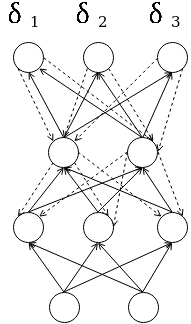
\includegraphics[scale=0.5]{backprop.png}
    \caption{La retropropagación en una red de tres capas. Las líneas sólidas muestran el paso
    del feedforward y las líneas discontinuas muestras la propagación hacia atrás de los valores $\delta$.}
    \label{fig:backprop}
\end{figure}
\paragraph{Actualización de los pesos}
Después de obtener las derivadas, el siguiente paso es actualizar los pesos
para disminuir el error. Como se dijo al principio, el término 
de retropropagación se refiere al método eficiente para calcular las 
derivadas $\frac{\partial E}{\partial w}$ y al algoritmo de optimización
que utiliza esas derivadas para ajustar los pesos y reducir el error.

La retropropagación como método de optimización es básicamente el 
descenso del gradiente. Sabemos que el gradiente negativo de $E$ apunta a la
dirección en la que $E$ se decrementa más rápido. Para minimizar $E$,
los pesos son ajustados en la dirección del gradiente negativo. La regla para
actualizar los pesos es

\[
w_{ij} \leftarrow  w_{ij} - \gamma \frac{\partial E}{\partial w_{ij}}
\]

donde la \textit{tasa de aprendizaje} $0 < \gamma$.
Hay dos variaciones básicas para la actualización, el \textit{modo por lotes} y 
\textit{en línea}.

\begin{itemize}
    \item \textbf{Aprendizaje por lotes}: En este modo, cada patrón $p$ es evaluado para obtener los términos de la derivada $\frac{\partial E_p}{\partial w}$; estos se suman para obtener la derivada total
    \[
      \frac{\partial E}{\partial w}  = \sum_p \frac{\partial E_p}{\partial w} 
    \]
    y sólo después de esto se actualizan los pesos. Los pasos son los siguientes:
    
    \begin{enumerate}
        \item Por cada patrón $p$ en el conjunto de entrenamiento
            \begin{itemize}
                \item Alimentar a la red con el patrón $p$ y hacer la propagación hacia adelante para obtener la salidas de la red.
                \item Calcular el error del patrón $E_p$ y retropropagar para obtener 
                las derivadas por patrón $\frac{\partial E_p}{\partial w}$.
            \end{itemize}
        \item Sumar todas las derivadas por patrón para obtener la derivada total.
        \item Actualizar los pesos
        \[
            w \leftarrow w - \gamma \frac{\partial E}{\partial w}
        \]
        \item Repetir.
    \end{enumerate}
    
    Cada paso a través de todo el conjunto de entrenamiento se llama \textit{época}.
    
    \item \textbf{Aprendizaje en línea}: En este modo de aprendizaje, los pesos
    se actualizan después de que se presenta cada patrón. Generalmente, un patrón $p$ se
    elige aleatoriamente y se presenta a la red. La salida se compara con el objetivo
    para ese patrón y los errores son propagados hacia atrás para obtener una
    derivada $\frac{\partial E_p}{\partial w}$  para un solo patrón. Los pesos se actualizan
    inmediatamente después, usando el gradiente del error de un solo patrón.
    Los pasos son:
    
    \begin{enumerate}
        \item Elegir aleatoriamente un patrón $p$ del conjunto de entrenamiento.
        \begin{itemize}
            \item Alimentar a la red con el patrón $p$ y propagar hacia adelante para
            obtener las salidas de la red.
            \item Calcular el error $E_p$ y retropropagar para obtener las derivadas $\frac{\partial E_p}{\partial w}$.
        \end{itemize}
        \item Actualizar los pesos usando la derivada de un solo patrón
        \[
            w \leftarrow w- \gamma \frac{\partial E_p}{\partial w}
        \]
        \item Repetir.
    \end{enumerate}
\end{itemize}


% Conviene primero calcular un valor $\delta_r$ para cada nodo $r$.

% \[
% \delta_r = \frac{\partial E_p}{ \partial h_r}
% \]

% La derivada para las aristas que conectan a las unidades ocultas y las de salida
% puede ser escrita como

% \begin{align*}\label{eq:hidden-output-derivative}
%     \frac{\partial E}{\partial w_{ij}} & = \frac{\partial E}{\partial o_i} \frac{\partial o_i}{\partial w_{ij}} \\
%     & =- (t_i - o_i) g'(h_i) v_j \\
%     & = \delta_i v_j
% \end{align*}

% definidos a  $\delta_i = -g'(h_i)(t_i - o_i)$.





% \subsubsection{El caso de redes con múltiples capas}


\subsubsection{Retropropagación en una forma matricial}

En estructuras de redes prealimentadas con múltiples capas, es conveniente 
reescribir el método de retropropagación en una forma
tal que las operaciones se simplifiquen a multiplicaciones
de vectores por matrices, matrices por vectores, matrices por matrices y vectores por vectores.
A continuación definiremos una red con dos capas, una oculta y una de salida, sin embargo,
se puede ver que es posible generalizar para redes con más capas ocultas. Todas las operaciones que se realizan son con respecto a una muestra $p$, por lo que
dependiendo de cómo se realice la actualización de los pesos, es como se
deben de realizar las operaciones con las matrices de las derivadas que obtendremos al final.


Consideraremos una red con $n$ unidades de entrada, $k$ unidades ocultas y $m$ unidades de salida. 
Hasta ahora la notación utilizada ha evitado que tratemos cada capa de una red
por separado, pero ahora es necesario mantener un índice de la capa sobre la que
se están haciendo los cálculo, por lo tanto se usa el superíndice $(l)$ para referirnos
a la capa $l$.
Los pesos entre la unidad de entrada $i$ y la oculta $j$ se denotan por $w_{ij}^{(1)}$. El peso 
entre la unidad oculta $i$ y la de salida $j$ será $w_{ij}^{(2)}$.

% El sesgo $b$ de cada unidad
% está implementado como el peso de una arista adicional. Por lo tanto, los vectores de entrada
% se extienden con un componente $1$, y lo mismo para el vector de salida de la capa oculta. 
% El peso entre la constante $1$ y la unidad oculta $j$ se llama $w_{n+1,j}^{(1)}$ y el peso
% entre la constante $1$ y la unidad de salida $j$ se denota por $w_{k+1, j}^{(2)}$.


Existen $n \times k$ pesos entre las unidades de entrada y las ocultas y
$k \times m$ entre las ocultas y las de salida. Sea $\mathbf{W_1}$ la matriz de
tamaño $n \times k$ cuyo componente $w_{ij}^{(1)}$ está en la $i$ ésima
fila y la $j$ ésima columna. De manera similar definamos $\mathbf{W}_2$ 
como la matriz de $k \times m$ con elementos $w_{ij}^{(2)}$. 
El vector de entrada es de tamaño $n$,  y lo definimos como $\mathbf{x} = (x_1, \dots, x_n)$. 

\begin{figure}
    \centering
    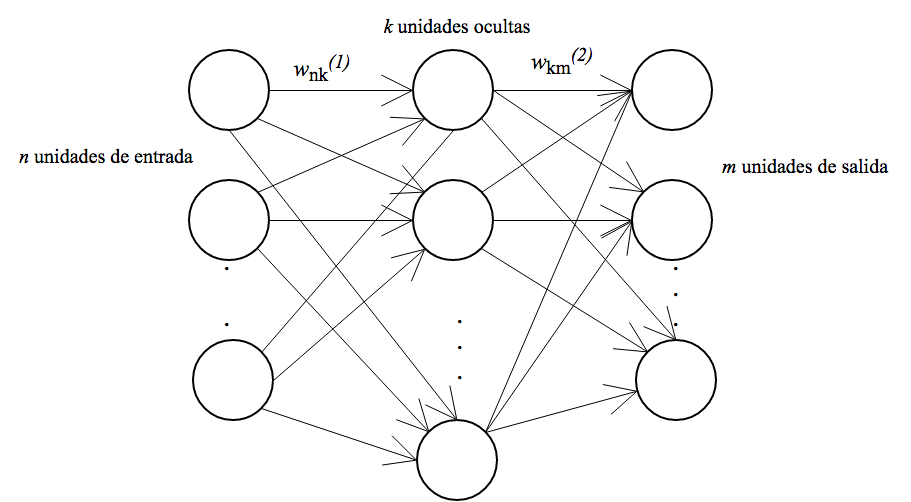
\includegraphics[scale=0.3]{mat_struct.png}
    \caption{Arquitectura de la red propuesta para la notación matricial de la retropropagación.}
    \label{fig:mat_mult_struct}
\end{figure}

Por ahora como función de activación usaremos a la sigmoide, por lo que la salida $y_j^{(1)}$ de la
unidad es

\[
y_j^{(1)} = f(\sum_{i}^{n} w_{ij}^{(1)}x_i) = \frac{1}{1+e^{\sum_{i}^{n} w_{ij}^{(1)}x_i}}
\]
 
Las salidas de la capa oculta se pueden obtener aplicando la función de activación a cada uno de los
elementos que resulten de la multiplicación
$\mathbf{x}\mathbf{W}_1$. El vector $\mathbf{y}^{(1)}$ cuyos componentes son las salidas de las unidades
ocultas está dado por

\[
\mathbf{y}^{(1)} = f(\mathbf{x}\mathbf{W}_1).
\]
Las salidas de las unidades en la capa de salida se calculan
usando el vector $\mathbf{y}^{(1)} = (y_1^{(1)},\dots, y_k^{(1)})$. La salida de la 
red es un vector $m$ dimensional $\mathbf{y}^{(2)}$, donde

\[
\mathbf{y}^{(2)} = f(\mathbf{y}^{(1)}\mathbf{W}_2).
\]

En el paso de feedforward, el vector $\mathbf{x}$ alimenta a la red.
Los vectores $\mathbf{y}^{(1)}$ y $\mathbf{y}^{(2)}$ son calculados.
Además, en este paso se pueden obtener las derivadas evaluadas 
de las funciones de activación, que se pueden escribir en matrices diagonales $\mathbf{D}_l$. Para nuestra red de dos capas,
$\mathbf{D}_2$ contiene las derivadas evaluadas de las funciones
de activación de los nodos de salida, y $\mathbf{D}_1$ para
las unidades ocultas. Por simplicidad, supusimos que $f$ es la sigmoide
y por lo tanto las derivadas son $f' = y(1-y)$.

\[
\mathbf{D}_2 = 
\begin{pmatrix}
    y_1^{(2)}(1-y_1^{(2)}) & 0 & \dots & 0 \\
    0 & y_2^{(2)}(1- y_2^{(2)}) & \dots & 0 \\
    \vdots & \vdots & \ddots & \vdots\\
    0 & 0 & \dots & y_m^{(2)}(1-y_m^{(2)}))
\end{pmatrix}
\]   
y


\[
\mathbf{D}_1 = 
\begin{pmatrix}
    y_1^{(1)}(1 - y_1^{(1)}) & 0 & \dots & 0 \\
    0 & y_2^{(1)}(1 - y_2^{(1)}) & \dots & 0 \\
    \vdots & \vdots & \ddots & \vdots\\
    0 & 0 & \dots & y_k^{(1)}(1 - y_k^{(1)}))
\end{pmatrix}
\]

Para calcular los valores delta de la unidad de salida
necesitamos las derivadas del error con respecto a las salidas. 
Definimos al vector $\mathbf{e}$ con las derivadas de las desviaciones cuadráticas como

\[
\mathbf{e} = 
\begin{pmatrix}
    - (t_1 - y_1^{(2)}) \\
    - (t_2 - y_2^{(2)}) \\
    \vdots \\
    - (t_m - y_m^{(2)})
\end{pmatrix}
\]

Para una unidad de salida  $\delta_i^{(2)} = - (t_i - y_i^{(2)})y_i^{(2)}(1- y_i^{(2)})$. Por lo tanto
el vector $m$ dimensional $\boldsymbol{\delta^{(2)}}$ que contiene todos los
valores delta de la unidad de salida está dado por

\[
\boldsymbol{\delta}^{(2)} = \mathbf{D}_2\mathbf{e}.
\]



El vector de tamaño $k$ de valores delta en la capa oculta es
\[
\boldsymbol{\delta}^{(1)} = \mathbf{D}_1\mathbf{W}_2 \boldsymbol{\delta}^{(2)}.
\]

Después de calcular los vectores con los valores delta, es posible
obtener las derivadas del error con respecto a los pesos.
Las matrices con las derivadas del error con respecto los pesos de $\mathbf{W}_2$
y $\mathbf{W}_1$, son respectivamente:

\[
\nabla \mathbf{W}_2 = (\boldsymbol{\delta}^{(2)}\mathbf{y}^{(1)})^T
\]
\[
\nabla \mathbf{W}_1 = (\boldsymbol{\delta}^{(1)}\mathbf{x})^T
\]

\[
\nabla\mathbf{W}_2 = 
\begin{pmatrix}
    \frac{\partial E}{w_{11}^{(2)}} & \dots & \frac{\partial E}{w_{1m}^{(2)}} \\
    \vdots & \ddots & \vdots\\
    \frac{\partial E}{w_{k1}^{(2)}} & \dots & \frac{\partial E}{w_{km}^{(2)}}
\end{pmatrix}
\]  

\[
\nabla\mathbf{W}_1 = 
\begin{pmatrix}
    \frac{\partial E}{w_{11}^{(1)}} & \dots & \frac{\partial E}{w_{1k}^{(1)}} \\
    \vdots & \ddots & \vdots\\
    \frac{\partial E}{w_{n1}^{(1)}} & \dots & \frac{\partial E}{w_{nk}^{(1)}}
\end{pmatrix}
\]  
Es fácil generalizar estas ecuaciones para $l$ capas de unidades de cómputo. Asumamos que la matriz
de conexión entre la capa $i$ e $i+1$ está denotada por $\mathbf{W}_{i+1}$. El vector
$\mathbf{\delta}^{(l)}$ de la capa de salida es entonces

\[
\boldsymbol{\delta}^{(l)} = \mathbf{D}_l\mathbf{e}
\]

El vector
$\mathbf{\delta}^{(i)}$ hasta la $i$ ésima capa se define recursivamente

\[
\boldsymbol{\delta}^{(i)} = \mathbf{D}_i\mathbf{W}_{i+1} \boldsymbol{\delta}^{(i+1)} \mbox{ para } i = 1, \dots, l - 1
\]

o de manera alternativa

\[
\boldsymbol{\delta}^{(i)} = \mathbf{D}_i\mathbf{W}_{i+1} \dots \mathbf{W}_{l-1}\mathbf{D}_{l-1}\mathbf{W}_l\mathbf{D}_{l} \mathbf{e}
\]

Las correcciones para las matrices de pesos se calculan de la misma manera que para las dos
capas de las unidades de cómputo.


% \paragraph{Pasos del algoritmo}. 

% La figura \ref{fig:extended_multilayer_net} muestra la red extendida para el cálculo de la función de costo. A modo de simplificar la
% explicación, trataremos con un solo par de entrada y salida $(\mathbf{o}, \mathbf{t})$ y se
% generalizará más tarde para $p$ muestras de entrenamiento. La red se ha extendido con una 
% capa de unidades adicional. El lado derecho calcula
% la desviación cuadrática $\frac{1}{2}(o_i^{(2)}- t_i)^2$ para el $i$ ésimo elemento del vector de salida
% y en el lado izquierdo se almacena $(o_i^{(2)} - t_i)$. Cada unidad de salida en red original
% calcula la función sigmoide $s$ y produce la salida $o_i^{(2)}$. La suma de las desviaciones
% cuadráticas nos da $E$. La función de costo para $p$ muestras de entrada y salida puede
% calcularse creando $p$ redes como la que mostramos, una por cada par de entrenamiento, y sumando
% las salidas de todas ellas para producir el error total del conjunto de entrenamiento.

% \begin{figure}
%     \centering
%     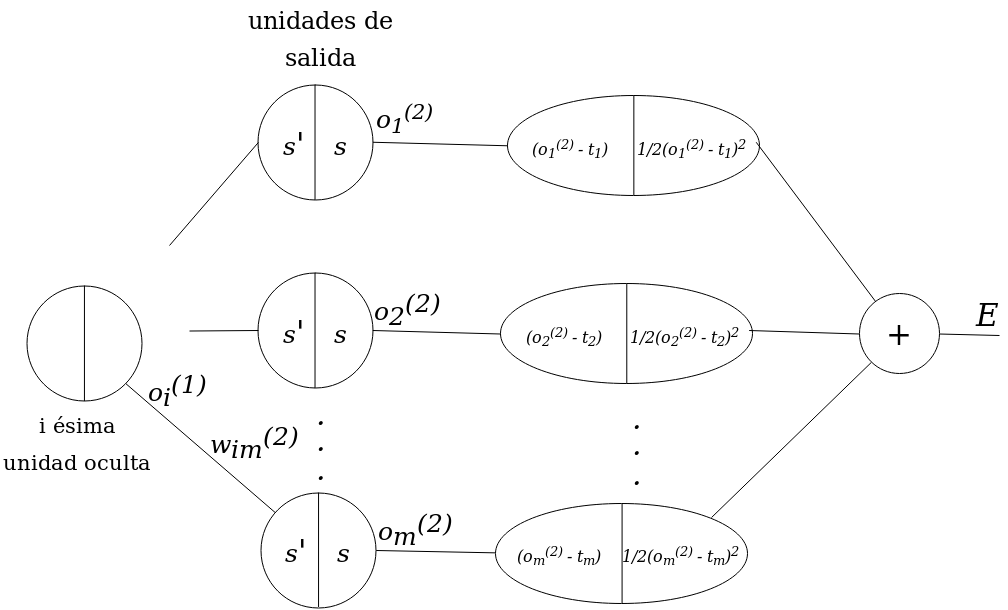
\includegraphics[scale=0.3]{extended_multilayer_network.png}
%     \caption{Red con múltiples capas extendida para el cáculo de $E$.}
%     \label{fig:extended_multilayer_net}
% \end{figure}

% Después de elegir los pesos de la red aleatoriamente, el algoritmo de propagación hacia atrás
% es usado para hacer las correcciones necesarias. El algoritmo puede descomponerse en los siguientes cuatro pasos:

% \begin{enumerate}
%     \item Cálculo feedforward
%     \item Retropropagación a la capa de salida
%     \item Retropropagación de la capa oculta
%     \item Actualización de pesos
% \end{enumerate}

% El algoritmo se detiene cuando el valor de la función de costo se ha vuelto lo suficientemente
% pequeño.

% \textbf{Primer paso: cálculo feedforward}. 

% \textbf{Segundo paso: retropropagación a la capa de salida}. Buscamos el primer
% conjunto de derivadas parciales $\frac{\partial E}{\partial w_{ij}^{(2)}}$. El camino de la 
% propagación hacia atrás desde la salida de la red hasta la unidad de salida $j$ se muestra
% en el diagrama B de la figura \ref{fig:backprop_output}.

% \begin{figure}
%     \centering
%     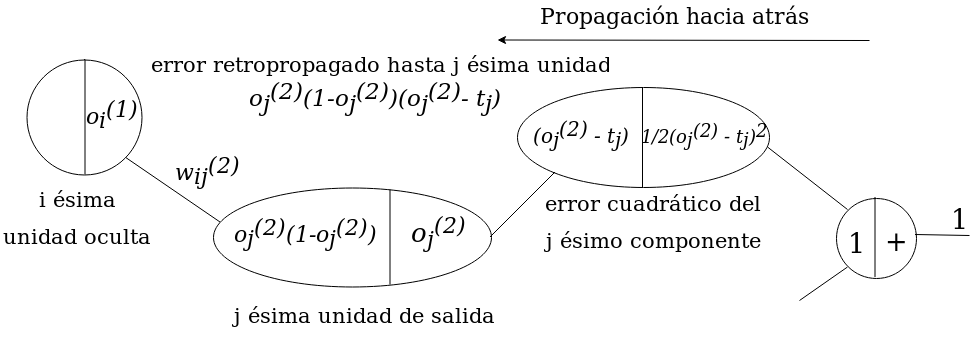
\includegraphics[scale=0.25]{backprop_hidden.png}
%     \caption{Camino de retropropagación hasta la unidad de salida $j$.}
%     \label{fig:backprop_output}
% \end{figure}

% Desde este camino se pueden recoger todos los términos multiplicativos que definen al
% error de retropropagación $\delta_j^{(2)}$. Por lo tanto

% \[
% \delta_j^{(2)}  = o_j^{(2)} (1-o_j^{(2)})(o_j^{(2)}-t_j)
% \]

% y la derivada parcial que buscamos es

% \[
% \frac{\partial E}{\partial w_{ij}^{(2)}} = [o_j^{(2)}(1-o_j^{(2)})(o_j^{(2)})(o_j^{(2)}-t_j)]o_j^{(1)} = \delta_j^{(2)}o_i^{(1)}
% \]

% Recordemos que para este último paso consideramos el peso $w_{ij}^{(2)}$ como una variables y su
% entrada $o_i^{(1)}$ una constante.

% En la figura \ref{fig:backprop_edge_multi_net} se muestra la situación general que encontramos durante el algoritmo
% de propagación hacia atrás. En el lado de la entrada de arista con peso $w_{ij}$
% tenemos $o_i^{(1)}$ y en el lado de la salida el error retropropagado $\delta_j^{(2)}$.

% \begin{figure}
%     \centering
%     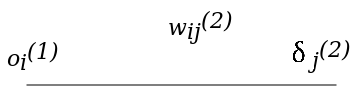
\includegraphics[scale=0.3]{backprop_edge.png}
%     \caption{Entrada y error retropropagado en una arista.}
%     \label{fig:backprop_edge_multi_net}
% \end{figure}

% \textbf{Tercer paso: retropropagación a la capa oculta}. Ahora queremos calcular las
% derivadas parciales $\frac{\partial E}{\partial w_{ij}^{(1)}}$. Cada unidad $j$ en la capa oculta
% está conectada a cada unidad $q$ en la capa de saida con una arista con pesos $w_{jq}^2$,
% para $q = 1, \dots, m$. El error retropropagado hasta la unidad $j$ en la capa oculta
% debe ser calculado tomando en cuenta todos los hacia atrás posibles, como se muestra en
% la figura \ref{fig:backprop_multi_net_input}. El error retropropagado es entonces

% \[
% \delta_j^{(1)} = o_j^{(1)} (1-o_j^{(1)}) \sum_{q=1}^m w_{jq}^{(2)}\delta_q^{(2)}
% \]

% Por lo tanto la derivada parcial que estamos buscando es

% \[
% \frac{\partial E}{\partial w_{ij}^{(1)}} = \delta_j^{(1)}o_i
% \]

% El error retropropagado puede ser calculado de la misma manera para
% cualquier número de capas ocultas y la expresión para las derivadas
% parciales de $E$ se mantiene la misma forma analítica.

% \begin{figure}
%     \centering
%     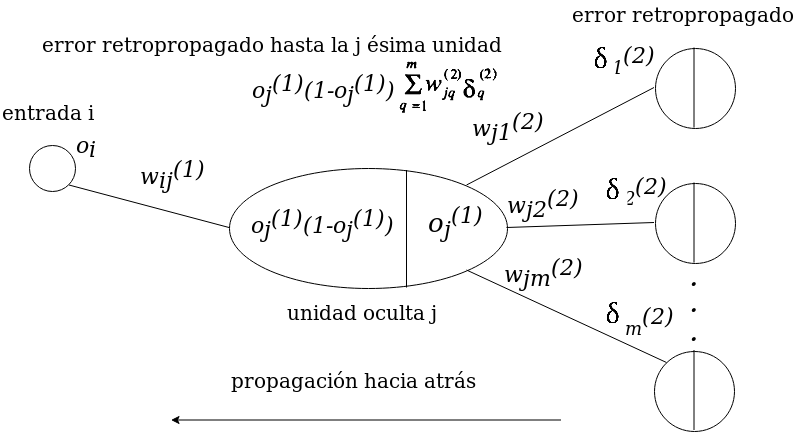
\includegraphics[scale=0.3]{backprop_input.png}
%     \caption{Todos los caminos hasta la entrada $i$.}
%     \label{fig:backprop_multi_net_input}
% \end{figure}


% \textbf{Cuarto paso: actualización de los pesos}. Después de calcular todas las derivadas
% parciales, los pesos de la red se actualizan en la dirección negativa del gradiente. Una
% constante de aprendizaje $\gamma$ define el tamaño del paso de la corrección. Las 
% correcciones para los pesos están dadas por

% \[
% \Delta w_{ij}^{(2)} = - \gamma o_i^{(1)}\delta_j^{(2)}, \mbox{ para }  i = 1, \dots, k+1; j = 1, \dots, m
% \]
% y

% \[
% \Delta w_{ij}^{(1)} = - \gamma o_i\delta_j^{(1)}, \mbox{ para }  i = 1, \dots, n+1; j = 1, \dots, k
% \]

% sabiendo que $o_{n+1} = o_{k+1}^{(1)} = 1$. Es muy importante hacer las
% correcciones de los pesos solamente después de haber calculado el error de retropropagación
% para todas las unidades en la red. De otro modo las correcciones se entrelazan con
% el error retropropagado y las correcciones calculadas ya no corresponden a la dirección del
% gradiente negativo. 

% \textbf{Más de una muestra de entrenamiento}. En el caso de $p > 1$ patrones de 
% entrada y salida, una red extendida se usa para calcular la función de costo
% para cada uno de ellos de manera separada. Las correcciones de los pesos se calculan
% para cada patrón y así obtenemos, por ejemplo, para el peso $w_{ij}^{(1)}$ las correcciones

% \[
% \Delta_1w_{ij}^{(1)}, \Delta_pw_{ij}^{(1)}, \dots, \Delta_pw_{ij}^{(1)}
% \]

% La actualizacion necesaria en la dirección del gradiente es entonces

% \[
% \Delta w_{ij}^{(1)} = \Delta_1w_{ij}^{(1)} + \Delta_2w_{ij}^{(1)} + \dots + \Delta_pw_{ij}^{(1)}
% \]

% Hablamos de actualizaciones \textit{offline} o por \textit{lotes} cuando la corrección
% de los pesos se hace de esta manera. Sin embargo, las actualizaciones de los pesos pueden hacerse
% secuencialmente después de presentar cada patrón, a esto se le llama entrenamiento \textit{online}.
% En este caso las correcciones no siguen exactamente la dirección del gradiente negativo,
% pero si los patrones de entrenamiento son seleccionados aleatoriamente la dirección de búsqueda
% oscila alrededor del la dirección exacta del gradiente y en la mayoría de los casos, el algoritmo
% implementa una forma de descenso en la función de costo. La razón de usar el entrenamiento
% online es que añade algo de ruido a la dirección del gradiente, lo que ayuda a evitar caer
% en mínimos locales de la función de costo. Además, cuando el conjunto de entrenamiento
% consiste en miles de patrones de entrenamiento, es muy costoso calcular la dirección 
% exacta del gradiente ya que cada \textit{época} (una ronda de presentación de todos
% los patrones de la red) consiste de muchos pasadas feedforward y el entrenamiento en
% línea se vuelve más eficiente.



% Hemos mostrado que en una red con una capa oculta y una de salida ($n, k$ y $m$ unidades)
% la entrada $\mathbf{o}$ produce la salida $\mathbf{o}^{(2)} = s(\mathbf{\hat{o}}^{(1)} \mathbf{W}_2)$
% donde $\mathbf{o}^{(1)} = s(\mathbf{\hat{o}}\mathbf{W}_1)$. En el paso de propagación hacia atrás sólo
% necesitamos las primeras $n$ filas de la matriz $\mathbf{W}_1$. Llamamos a esta matriz de $n \times k$, 
% $\mathbf{\overline{W}}_1$. Similarmente, a la matriz de $k \times m$ $\mathbf{\overline{W}}_2$
% compuesta por las primeras $k$ filas de la matriz $\mathbf{W}_2$. Asumimos esto porque no necesitamos 
% propagar hacia atrás valores  hacia las entradas constantes que corresponden a cada
% sesgo.

% Las derivadas almacenadas en el paso de feedforward en las $k$ unidades ocultas y
% las $m$ unidades de salida pueden ser escritas como las siguientes dos matrices diagonales. 
% Suponemos que nuestra función de activación en todas las unidades es la sigmoide.


% Definimos al vector $\mathbf{e}$ con las derivadas de las desviaciones cuadráticas como

% \[
% \mathbf{e} = 
% \begin{pmatrix}
%     (o_1^{(2)} - t_1) \\
%     (o_2^{(2)} - t_2) \\
%     \vdots \\
%     (o_m^{(2)} - t_m)
% \end{pmatrix}
% \]

% El vector $m$ dimensional $\boldsymbol{\delta^{(2)}}$ del error retropropagado hasta las 
% unidades de salida está dado por la expresión

% \[
% \boldsymbol{\delta}^{(2)} = \mathbf{D}_2\mathbf{e}
% \]


\subsection{Aprendizaje profundo}
El \textit{aprendizaje profundo} permite a las computadoras construir conceptos complejos
a partir de conceptos más simples. La figura 
\ref{fig:deeplearning_person} muestra como un sistema de aprendizaje profundo
puede representar el concepto de la imagen de una persona al combinar conceptos más simples, tales
como esquinas y contornos, que a su vez están definidos en términos de los bordes.
El ejemplo por excelencia de un modelo de aprendizaje profundo es una \textit{red neuronal feedforward
profunda}, donde que sea profunda significa que tiene dos o más capas ocultas. Una red neuronal
es simplemente una función matemática que mapea algún conjunto de valores de entrada en 
valores de salida. La función está formada por una composición de funciones más simples.
Podemos suponer que al aplicar cada función matemática se obtiene una nueva representación de la
entrada.\\

\begin{remark}

El aprendizaje profundo es un tipo de aprendizaje automático
poderoso y flexible que aprende una representación del mundo
como una jerarquía anidada de conceptos, donde 
cada concepto está definido a partir de conceptos más simples,
y representaciones más abstractas calculadas en términos
de menos abstractas.

\end{remark}


\begin{figure}
    \centering
    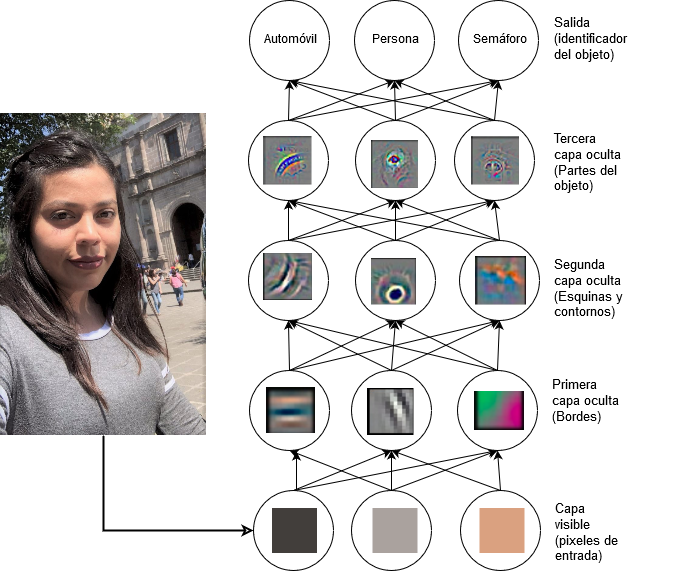
\includegraphics[scale=0.5]{figures/deep_learning_person.png}
    \caption{Ejemplo de un modelo de aprendizaje profundo. El aprendizaje profundo resuelve el problema de mapear un conjunto de pixeles al identificador de un objeto separando este mapeo
    complejo en mapeos simples anidados, cada uno descrito por
    una capa diferente en el modelo. La entrada es presentada
    en la capa visible, llamada así porque contiene las variables que somos capaces de observar. Después una serie de capas ocultas extraen de la imagen características cada vez más
    abstractas. Estas capas se llaman \textit{ocultas} porque
    sus valores no son dados en los datos; en su lugar, el modelo
    debe determinar qué conceptos son útiles para explicar 
    las relaciones de los datos observados. Dados los pixeles,
    la primera capa puede fácilmente identificar bordes comparando
    el brillo entre vecindades de pixeles.
    Dada la descripción de bordes de la primera capa, la segunda
    capa puede con facilidad buscar esquinas y contornos
    que son reconocibles como colecciones de bordes. Dada el 
    resultado de la segunda capa oculta, la tercera capa detecta
    partes enteras de objetos específicos, al encontrar
    colecciones específicas de contornos y esquinas. 
    Finalmente, esta descripción de la imagen en términos 
    de partes de objetos puede ser usada para reconoces objetos
    presentes en la imagen.\label{fig:deeplearning_person}}
    
\end{figure}
% La idea del aprender la representación correcta de los datos provee una perspectiva del aprendizaje
% profundo. Otra perspectiva sobre el aprendizaje profundo es que la profundidad permite a la
% computadora aprender un programa de varias etapas. Cada capa de la representación puede
% ser el estado de la memoria de la computadora después de ejecutar un conjunto de instrucciones
% en paralelo. Las redes con una profundidad mayor puede correr más instrucciones en secuencia. Las
% instrucciones en secuencia son poderosas porque instrucciones posteriores pueden hacer referencia
% a resultados de instrucciones previas. De acuerdo a este enfoque del aprendizaje profundo, no toda
% la información en las activaciones de una capa necesariamente codifica los factores de variación que
% explican la entrada. La representación también almacena información de estados que ayudan a la
% ejecución de un programa que puede dar sentido a la entrada. Esta información de estado puede ser
% análogo a un contador o a un apuntador en un programa de computadora tradicional. No tiene
% nada que ver con el contenido de la entrada específicamente, pero permite que el modelo
% se organice para su procesamiento.

% Hay dos maneras de medir la profundidad de un modelo. La primera es basándose en el número de 
% instrucciones secuenciales que deben ejecutarse para evaluar la arquitectura. 


\subsection{Redes neuronales convolucionales}

\begin{remark}
Las redes neuronales convolucionales o CNN (por sus siglas en inglés), son un tipo especializado
de red neuronal para procesamiento de datos que tienen una topología parecida a una cuadrícula. El nombre de 
red convolucional indica que la red ocupa una operación matemática llamada convolución. Las redes 
neuronales
convolucionales son simplemente redes neuronales que usan la convolución en lugar de la multiplicación de 
matrices en al menos una de sus capas.
\end{remark}


Las redes convolucionales son una categoría dentro de las redes neuronales profundas, que han 
demostrado ser muy efectivas en áreas como el reconocimiento y clasificación de imágenes. Debido
a los excelentes resultados de las CNN en estas áreas, nos enfocaremos en estas redes para tareas
de visión computacional.\\

% \subsubsection{La operación de convolución}
% Consideremos un filtro de dos dimensiones (también llamado máscara o kernel),
% $w(x, y)$, de tamaño $m \times n$. La correlación del filtro con una imagen $f(x,y)$,
% denotada como $w(x,y) \star f(x,y)$, está dada por:

% \begin{equation}\label{correlation}
%     w(x,y) \star f(x,y) = \sum_{s=-a}^a \sum_{t=-b}^b w(s,t)f(x+s, y+t)
% \end{equation}
% . Convolucionar el filtro con una imagen $I(n_1, n_2)$
% y producir la imagen $Z(n_1, n_2)$ se representa como sigue:

% \begin{equation*}
%     Z(n_1, n_2) = \sum_{l=0}^a\sum_{w=0}^b F(l, w) I(n_1+l, n_2+w) \forall n_1, n_2
% \end{equation*}

\begin{remark}
La correlación es una operación que funciona recorriendo una imagen y aplicando un
\textit{filtro} a cada pixel. El filtro se denota como un \textit{kernel}. Primero 
el kernel se llena con números llamados coeficientes de kernel. Estos coeficientes 
ponderan el valor del pixel que cubren y la salida de la correlación es la suma
de los valores de los pixeles ponderados. Matemáticamente la correlación de la imagen
$I$ con el kernel $K$ se puede expresar como sigue:
\begin{equation}\label{correlation}
    S(i,j) = (I * K)(i,j) = \sum_{m} \sum_{n} I(i+m, j+n) K(m,n).
\end{equation}
\end{remark}

% donde $m$ y $n$ son el largo y ancho del kernel respectivamente.
La correlación está asociada con el término de \textit{convolución} y ambos se utilizan
en el contexto de procesamiento de imágenes. La convolución únicamente difiere en la manera
en que el kernel se aplica a la imagen. Formalmente la convolución se define como:

\[
S(i,j) = \sum_{m} \sum_{n} I(i-m, j-n) K(m,n).
\]

Comparando esta ecuación con la de correlación (ecuación \ref{correlation}), podemos
ver que las únicas diferencias son los signos negativos. La interpretación de esto
es que el kernel está rotado $180$ grados antes de hacer la correlación.

Cuando se aplica un filtro para suavizar una imagen, encontrar bordes, etcétera, el 
proceso se denota como convolución incluso si se implementa como una correlación. Por
lo tanto, por conveniencia llamaremos a ambas operaciones convolución.

\begin{figure}[htbp]
    \centering
    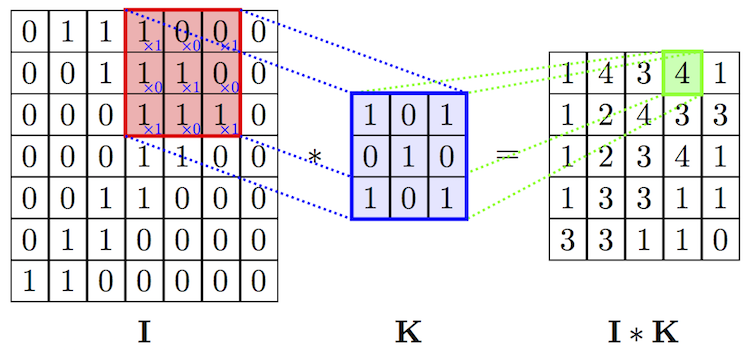
\includegraphics[scale=0.5]{conv_operation.png}
    \caption{Convolución entre una imagen
    $I$ y un kernel $K$ sin rotarlo 180 grados.}
    \label{fig:convolution_example}
\end{figure}

En la figura \ref{fig:convolution_example} para calcular
cada valor en la salida, el kernel se mueve con un paso 
de tamaño uno sobre el eje horizontal y vertical. Este paso
se conoce como \textit{zancada} o \textit{stride} (en inglés).
El valor de la zancada puede ser diferente de uno, según 
convenga. El tamaño de $I * K$ para una imagen $I$ de tamaño
$h \times w$ y un filtro de tamaño $f \times f$ depende también de
la zancada $s$.

\[
h' = \lfloor\frac{h-f+s}{s}\rfloor
\]

\[
w' = \lfloor\frac{w-f+s}{s}\rfloor
\]

donde $h'$ y $w'$ son las dimensiones del resultado.
Se puede notar que entre más grande sea el valor de $s$
el tamaño de $I * K$ disminuye. Sin embargo, en algunas 
aplicaciones es necesario conservar el tamaño de la entrada.
Esto último se logra aplicando un \textit{borde de ceros}
a la imagen de entrada. Al añadir el borde de ceros las
dimensiones el tamaño del resultado de la convolución se 
incrementa. Si $p$ denota el incremento sobre cada dimensión
de $I$, el tamaño de $h'$ y $w'$ se calculan de la siguiente 
forma:


\[
h' = \lfloor\frac{h-f+s+p}{s}\rfloor
\]

\[
w' = \lfloor\frac{w-f+s+p}{s}\rfloor
\]

% \subsubsection{Motivación}

La convolución aprovecha dos ideas importantes que pueden ayudar a mejorar un
sistema de aprendizaje automático: \textit{interacciones escasas} y \textit{compartición de parámetros}.

Las capas de las redes neuronales tradicionales usan la multiplicación de matrices de parámetros con
un parámetro separado entre cada unidad de entrada y cada unidad de salida. Esto significa que cada 
unidad de salida interactúa con cada unidad de entrada. Las redes convolucionales, sin embargo, 
tienen \textit{interacción escasa} (también conocida como 
conectividad escasa o pesos escasos). Esto se logra haciendo que el kernel sea de menor
tamaño que la entrada. Por ejemplo, cuando se procesa una imagen, la imagen de entrada puede tener 
miles o millones de pixeles, pero podemos detectar pequeñas y significativas características como
bordes con kernels que sólo ocupan decenas o cientos de pixeles. En consecuencia se puede ver
que se almacenan menos parámetros, lo que reduce los requisitos de memoria del modelo 
y mejora la eficiencia estadística. Además significa que el cálculo de las salidas requiere menos 
operaciones.

La \textit{compartición de parámetros} se refiere a usar el mismo parámetro para más de una función
en un modelo. En una red neuronal tradicional, cada elemento de la matriz de pesos se usa 
exactamente una vez cuando se calcula la salida de una capa. Se multiplican por un elemento en la 
entrada y nunca se vuelve a visitar. En una CNN, cada elemento del kernel se usa en cada posición de la
entrada. La compartición de parámetros indica que más que aprender un conjunto de parámetros 
por separado para cada posición, aprendemos sólo un conjunto. 


Sabemos que cada kernel puede verse como una cuadrícula de números también llamados pesos
y que éstos se aprenden durante el entrenamiento de la CNN. El proceso de aprendizaje involucra 
la inicialización de los pesos del kernel al comenzar el entrenamiento. Posteriormente, dados los pares
de entrada-salida, los pesos son ajustados en varias iteraciones durante el proceso de aprendizaje.\\

\begin{remark}
Un capa típica en una CNN consiste de tres etapas. En la 
primera etapa, la capa realiza diferentes convoluciones en
paralelo para producir una colección de mapas de
características. En la segunda etapa cada mapa 
de características se pasa por una función de activación
no lineal. La función de activación más común es el 
rectificador o ReLU definido como $g(z) = max(0, z)$.
Esta etapa también se conoce como detector.
En la tercera etapa utilizamos una función de agrupación
o pooling para modificar la salida de la capa aún más.
\end{remark}

\begin{remark}
Una función de pooling reemplaza la salida de la red en cierta
ubicación con una estadística resumida de las salidas vecinas.
Por ejemplo, la operación de agrupamiento máximo
retorna el valor máximo dentro de una vecindad rectangular.
\end{remark}


El agrupamiento ayuda a hace que la representación se vuelva 
aproximadamente invariante a pequeñas traslaciones de
la entrada. La \textit{invarianza a las traslaciones} significa 
que si trasladamos la entrada por una pequeña cantidad, los
valores de la mayoría de las salidas agrupadas no cambian.
La invarianza a traslaciones locales puede ser muy útil cuando
nos importa si una característica está presente y no 
exactamente donde.

A las capas que pasan por las tres etapas las llamaremos \textit{capas
de convolución}, aunque para algunos autores, cada etapa es una capa
diferente, la primera es de convolución, la segunda de pooling y la 
tercera de no linealidad. Por simplicidad elegimos el término
de capa de convolución.

% La capa de convolución es el componente más importante de una CNN. Esta capa realiza la 
% convolución entre un conjunto de kernels y la entrada de la capa para producir como salida
% un colección de \textit{mapas de características}, donde cada uno de éstos es el resultado
% de la convolución entre un kernel y la entrada.


% \subsubsection{Pooling}

% \subsubsection{ReLU}
% En redes neuronales modernas, la función de activación estándar recomendada (principalmente
% para tareas de visión)
% es la \textit{unidad lineal rectificada} o ReLU (por sus siglas en inglés).
% Esta función mapea la entrada a $0$ si es negativa y mantiene el valor original
% si es positiva. Esto se representa como sigue

% \[
% f (x) = \max(0,x)
% \]

% \subsubsection{Entropía cruzada}

% La función de costo para una red convolucional se elige dependiendo
% de la tarea que se desea realizar. Por ejemplo, hasta ahora hemos utilizado
% la suma de errores cuadráticos; esta función se utiliza en tareas de
% regresión. Para tareas de clasificación en múltiples clases usamos como función de
% costo la \textit{entropía cruzada} definida como

% \[
% E_{log} = -\sum_p \sum_i t_{pi} \log(y_{pi})
% \]

% donde $y_{pi}$ es la probabilidad estimada de que el patrón $p$ que pertenezca
% a la clase $i$ y $t_{pi} \in \{0,1\}$ es el objetivo.

% La probabilidad de cada clase para un patrón $p$ puede ser calculada usando la función
% \textit{softmax}:

% \[
% y_{i} = \frac{e^{\hat{y}_i}}{\sum_k e^{\hat{y}_k}}
% \]

% donde $\hat{y}_i$ es la salida de la red de la unidad $i$ y la suma es sobre las 
% $k$ unidades de salida.

% \subsubsection{Dropout}

% Un problema central en el aprendizaje automático es cómo hacer que un algoritmo
% se desempeñe bien no sólo en el conjunto de entrenamiento, sino también con
% nuevos patrones de entrada. Muchas estrategias usadas en el aprendizaje automático están 
% diseñadas para reducir el error de prueba. Estas estrategias se conocen colectivamente 
% como \textit{regularización}.

% Definimos la regularización como cualquier modificación que hacemos a nuestro algoritmo de 
% aprendizaje con la intención de reducir el error de generalización pero no 
% el error de entrenamiento.

% Una de las estrategias más populares para la regularización de redes neuronales es
% el \textit{dropout}. Específicamente el dropout entrena el conjunto de todas las subredes que pueden
% ser formadas al remover las unidades que no son de salida a partir de una red base.
% % Consideremos una red neuronal completamente conectada compuesta por $L$ capas e indexadas por
% % $l $
% Para entrenar con dropout utilizamos un algoritmo de aprendizaje
% basado en lotes. Cada vez que tomamos una muestra del lote, aleatoriamente 
% muestreamos una máscara binaria que se aplica a todas las unidades ocultas y de
% entrada en la red. La máscta para cada unidad se muestrea independientemente de todas las
% demás. La probabilida de tomar una máscara con calor uno (causando que la unidad se incluya)




% \subsubsection{Convolución}
% \subsubsection{Pool}

% \subsubsection{ReLU}
% \subsubsection{Softmax}

% \subsection{Otros conceptos}
% \subsubsection{Entropía cruzada}
% \subsubsection{Dropout}
% \subsubsection{One-hot encoding}

\subsection{TensorFlow}

TensorFlow es una biblioteca de código abierto para computo numérico. Fue desarrollada 
originalmente por investigadores e ingenieros del equipo de Google Brain, con 
el propósito de motivar la investigación de arquitecturas profundas.

TensorFlow es una interfaz para expresar algoritmos de aprendizaje automático
y una implementación para ejecutar tales algoritmos.
Un cálculo expresado en TensorFlow puede ser ejecutado con ningún o con mínimos
cambios en una amplia variedad de sistemas desde dispositivos móviles
como teléfonos o tabletas hasta sistemas distribuidos a gran escala
de cientos de máquinas y cientos de dispositivos con unidades de procesamiento 
gráfico (GPU). El sistema es flexible y puede usarse para expresar una gran 
variedad de algoritmos, incluyendo algoritmos de entrenamiento
e inferencia para modelos de redes neuronales profundas y ha sido usado
para llevar a cabo investigaciones en áreas como la visión computacional,
robótica, procesamiento de lenguaje natural, etcétera.\\ 

\begin{remark}
Los cálculos en TensorFlow son descritos por una gráfica dirigida
que está compuesta por un conjunto de nodos y aristas.
La gráfica representa un cálculo de flujo de datos (un modelo
de programación para cómputo paralelo).
\end{remark}
A menudo los clientes construyen la gráfica de cómputo usando uno de los
lenguajes de frontend soportados (C++ o Python). Todos los ejemplos
que se muestran en esta sección están desarrollados en Python.

En una gráfica de TensorFlow los nodos representan instancias de \textit{operaciones}, éstos tienen cero o más entradas y
cero o más salidas. Los valores que fluyen sobre las aristas en la gráfica son
\textit{tensores}. Estos últimos son arreglos de dimensiones arbitrarias donde el tipo
de sus elementos se especifica o infiere durante la construcción de la gráfica.

Una \textit{operación} tiene un nombre y representa un cálculo abstracto, por ejemplo,
una multiplicación de matrices o una suma. 

Los programas clientes interactúan con el sistema de TensorFlow creando una
\textit{Session}. El objeto Session es una interfaz para la gráfica de cómputo,
es quien permite su ejecución a través de su operación primaria
\textit{Run}, la cual toma un conjunto de nodos de la gráfica que necesitan ser
calculados, así como un conjunto de tensores que necesitan alimentar a la 
gráfica para poder obtener las salidas de ciertos nodos. TensorFlow puede calcular
la cerradura transitiva de todos los nodos que deben ser ejecutados
para poder calcular las salidas que fueron solicitadas en los argumentos de \textit{Run}.

\begin{quote}
\begin{savenotes}\sphinxattablestart
\centering
\sphinxcapstartof{table}
\caption{Algunos de los tipos de operaciones en TensorFlow.}\label{\detokenize{chapter_one/tensorflow:operations}}
\sphinxaftercaption
%\begin{tabulary}

%%%%%%%%%%%%%%%5
\begin{tabulary}{\linewidth}[t]{|T|T|}
%\begin{tabulary}[t]{|c|c|}
\hline 
Categoría & Ejemplo \\ 
\hline 
Operaciones matemáticas a nivel de elementos & \texttt{Add, Sub, Mul, Div, Exp, Log, Greater, Less, Equal, ...} \\ 
\hline 
Operaciones con arreglos & \texttt{Concat, Slice, Split, Constant, Rank, Shape, Shuffle, ...} \\ 
\hline 
Operaciones con matrices & \texttt{MatMul, MatrixInverse, MatrixDeterminant, ...} \\ 
\hline 
Construcción de redes neuronales & \texttt{SoftMax, Sigmoid, ReLU, Convolution2D, MaxPool} \\ 
\hline 
Operaciones de puntos de control & \texttt{Save, Restore} \\ 
\hline 
\end{tabulary} 

%%%%%%%%%%%%%%%%5
% \end{tabulary}
\par
\sphinxattableend\end{savenotes}
\end{quote}
\subsubsection{Variables}

Cuando construimos un modelo de aprendizaje en TensorFlow utilizamos \textit{variables}
para representar los parámetros del modelo. Las variables de TensorFlow
son buffers en memoria que contienen tensores; pero a diferencia de los tensores
normales que sólo son instanciados cuando una gráfica se ejecuta y que 
inmediatamente después se eliminan, las variables se mantienen durante
múltiples ejecuciones de una gráfica. Como resultado, las variables de TensorFlow 
tienen las siguientes tres propiedades:

\begin{itemize}
\item Las variables deben inicializarse explícitamente antes de que una gráfica
se utilice por primera vez.
\item Podemos utilizar métodos de optimización como el del descenso del gradiente 
para modificar las variables después de cada iteración para ajustar los 
parámetros óptimos del modelo.
\item Podemos guardar en el disco los valores de las variables y restaurarlos
para su uso posterior.

\end{itemize}

Crear e inicializar una variable es muy simple,
únicamente utilizamos la clase \sphinxcode{Variable}
dentro de la biblioteca de TensorFlow.
Comencemos por inicializar una variable
que describe los pesos entre dos capas en una red neuronal.

\begin{sphinxVerbatim}[commandchars=\\\{\}]
\PYG{n}{weights} \PYG{o}{=} \PYG{n}{tf}\PYG{o}{.}\PYG{n}{Variable}\PYG{p}{(}\PYG{n}{tf}\PYG{o}{.}\PYG{n}{random\PYGZus{}normal}\PYG{p}{(}\PYG{p}{[}\PYG{l+m+mi}{300}\PYG{p}{,} \PYG{l+m+mi}{200}\PYG{p}{]}\PYG{p}{,} \PYG{n}{stddev}\PYG{o}{=}\PYG{l+m+mf}{0.5}\PYG{p}{)}\PYG{p}{,}
\PYG{n}{name}\PYG{o}{=}\PYG{l+s+s2}{\PYGZdq{}}\PYG{l+s+s2}{weights}\PYG{l+s+s2}{\PYGZdq{}}\PYG{p}{)}
\end{sphinxVerbatim}

\sphinxcode{tf} es un alias para el módulo \sphinxcode{tensorflow}.
\sphinxcode{tf.Variable} recibe dos argumentos; el primero,
\sphinxcode{tf.random\_normal}, que es una operación que
produce un tensor inicializado usando una
distribución normal con una desviación estándar de
0.5 y media 0. El tamaño del tensor es de $300 \times
200$, lo que significa que los pesos conectan a una
capa de 300 neuronas a una de 200. El segundo
parámetro es un identificador único que nos
permite referirnos a un nodo en específico en
la gráfica de cómputo.

Por defecto las variables son entrenables,
lo que quiere decir que cuando utilizamos un método
como el descenso del gradiente, las variables
automáticamente cambian sus valores.


\subsubsection{Placeholder}

Los modelos de aprendizaje necesitan una entrada ya sea 
para el entrenamiento o la evaluación. Una variable no es 
suficiente porque sólo se inicializa una vez. Necesitamos un
componente que llenemos cada que la gráfica de cómputo se ejecuta.
TensorFlow usa una estructura llamada \textit{placeholder}. 

Un placeholder es instanciado como sigue y puede ser utilizado en operaciones como los tensores
y variables en TensorFlow.

\begin{sphinxVerbatim}[commandchars=\\\{\}]
\PYG{n}{x} \PYG{o}{=} \PYG{n}{tf}\PYG{o}{.}\PYG{n}{Placeholder}\PYG{p}{(}\PYG{n}{tf}\PYG{o}{.}\PYG{n}{float32}\PYG{p}{,} \PYG{n}{name}\PYG{o}{=}\PYG{l+s+s2}{\PYGZdq{}}\PYG{l+s+s2}{x}\PYG{l+s+s2}{\PYGZdq{}}\PYG{p}{,} \PYG{n}{shape}\PYG{p}{[}\PYG{k+kc}{None}\PYG{p}{,} \PYG{l+m+mi}{1024}\PYG{p}{]}\PYG{p}{)}
\PYG{n}{W} \PYG{o}{=} \PYG{n}{tf}\PYG{o}{.}\PYG{n}{Variable}\PYG{p}{(}\PYG{n}{tf}\PYG{o}{.}\PYG{n}{random\PYGZus{}uniform}\PYG{p}{(}\PYG{p}{[}\PYG{l+m+mi}{784}\PYG{p}{,}\PYG{l+m+mi}{10}\PYG{p}{]}\PYG{p}{,} \PYG{o}{\PYGZhy{}}\PYG{l+m+mi}{1}\PYG{p}{,} \PYG{l+m+mi}{1}\PYG{p}{)}\PYG{p}{,} \PYG{n}{name}\PYG{o}{=}\PYG{l+s+s2}{\PYGZdq{}}\PYG{l+s+s2}{W}\PYG{l+s+s2}{\PYGZdq{}}\PYG{p}{)}
\PYG{n}{multiply} \PYG{o}{=} \PYG{n}{tf}\PYG{o}{.}\PYG{n}{matmul}\PYG{p}{(}\PYG{n}{x}\PYG{p}{,} \PYG{n}{W}\PYG{p}{)}
\end{sphinxVerbatim}

En el ejemplo definimos un placeholder donde \sphinxcode{x}
representa un lote de datos de tipo \sphinxcode{float32}.
Podemos notar que \sphinxcode{x} tiene 1024 columnas, lo
que significa que cada patrón de entrada
tiene una dimensión de 1024. Se puede notar también
que \sphinxcode{x} tiene un número indefinido de filas.
Esto significa que \sphinxcode{x} puede ser inicializado
con un número arbitrario de muestras. Aunque podemos
multiplicar cada muestra por separado con \sphinxcode{W},
al expresar un lote completo como un tensor tenemos
permitido calcular los resultados de todas los
patrones de entrada en paralelo. El
resultado de la fila $i$ del tensor de
multiplicación corresponde a multiplicar \sphinxcode{W}
con el patrón $i$.

Así como las variables se inicializan la primera vez
que se construye la gráfica, los placeholder necesitan
llenarse cada vez que se ejecuta la gráfica o una
subgráfica de cómputo.


\subsubsection{Ejemplo de una red neuronal en TensorFlow}

En este apartado se describe la creación de un modelo de aprendizaje muy
simple, una red neuronal, en TensorFlow para el cálculo de la función
\textbf{XOR}.


Como estamos en el contexto del aprendizaje automático
supervisado, necesitamos un conjunto de datos etiquetado.
Nuestro conjunto de datos está dado por la tabla \ref{table:xor}. Las
primeras dos columnas son los atributos $X_1$ y $X_2$ y la tercera 
columna es el objetivo.


\begin{quote}
\begin{savenotes}\sphinxattablestart
\centering
\sphinxcapstartof{table}
\caption{Definición de la función XOR.\label{table:xor}}
\sphinxaftercaption
\begin{tabulary}{\linewidth}[t]{|T|T|T|}
\hline 
$X_1$ & $X_2$ & $Y = X_1 \oplus X2$ \\ 
\hline 
0 & 0 & 0 \\ 
\hline 
1 & 0 & 1 \\ 
\hline 
0 & 1 & 1 \\ 
\hline 
1 & 1 & 0 \\ 
\hline 
\end{tabulary} 
\par
\sphinxattableend\end{savenotes}
\end{quote}


La arquitectura de nuestra red es la siguiente: una capa de entrada con dos unidades
de entrada $X_1$ y $X_2$. Una capa oculta con dos unidades, que tienen como función
de activación la sigmoide. Por último una unidad de salida con la función sigmoide.
De manera gráfica esto se puede ver en la figura \ref{image:xor_net}.

\begin{figure}[ht]
\centering
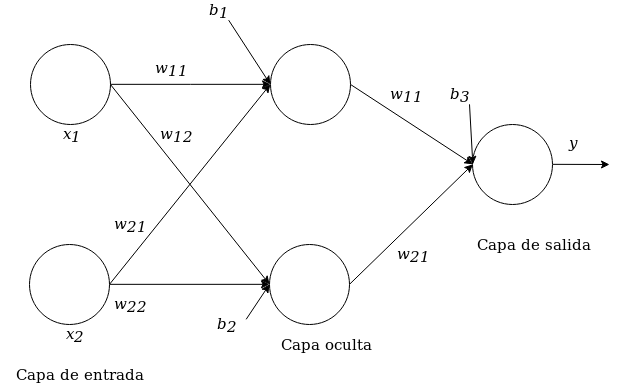
\includegraphics[scale=0.5]{xor_net.png}
\caption{\label{image:xor_net} Arquitectura de la red neuronal para calcular la función $\oplus$.}
\end{figure} 

Antes de comenzar con el código conviene dibujar la gráfica de cómputo que
deseamos ejecutar.
La gráfica de cómputo está descrita en la figura \ref{fig:xor_graph}.
Los círculos representan o variables o placeholders excepto para
la salida predicha $y'$ que es el resultado de una operación. Tenemos
un placeholder para 
las entradas $X$ y otro para las salidas correctas u objetivos $y$. Las variables
son los pesos $W_i$ y los sesgos $b_i$.
Los rectángulos son las operaciones. En una red neuronal las únicas operaciones
son la multiplicación y suma de tensores, la aplicación de la función de
activación y un método de optimización como el descenso del gradiente para
minimizar el error dado por una función de costo, en nuestro caso
la suma de errores cuadráticos (SSE). 
Durante la ejecución de la gráfica las variables cambiarán su valor
automáticamente a los valores óptimos que minimicen el error.

\begin{figure}[ht]
\centering
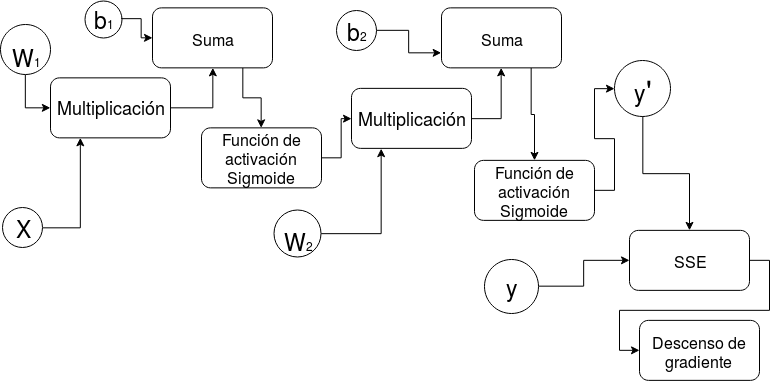
\includegraphics[scale=0.45]{xor_tf_graph.png}
\caption{\label{fig:xor_graph}La gráfica de TensorFlow que representa a la arquitectura de la red para
el cálculo de la función $\oplus$.}
\end{figure}


Un programa en TensorFlow se compone de dos partes,
la creación de la gráfica y su ejecución.

Antes que nada como para cualquier biblioteca, se importa \sphinxcode{tensorflow}.

\begin{sphinxVerbatim}[commandchars=\\\{\}]
\PYG{k+kn}{import} \PYG{n+nn}{tensorflow} \PYG{k}{as} \PYG{n+nn}{tf}
\end{sphinxVerbatim}

El conjunto de datos se puede definir en dos listas, una con los datos
de entrada y la otra con sus respectivas salidas.

\begin{sphinxVerbatim}[commandchars=\\\{\}]
\PYG{n}{datos\PYGZus{}de\PYGZus{}entrada} \PYG{o}{=} \PYG{p}{[}\PYG{p}{[}\PYG{l+m+mf}{0.}\PYG{p}{,} \PYG{l+m+mf}{0.}\PYG{p}{]}\PYG{p}{,} \PYG{p}{[}\PYG{l+m+mf}{1.}\PYG{p}{,} \PYG{l+m+mf}{0.}\PYG{p}{]}\PYG{p}{,} \PYG{p}{[}\PYG{l+m+mf}{0.}\PYG{p}{,} \PYG{l+m+mf}{1.}\PYG{p}{]}\PYG{p}{,} \PYG{p}{[}\PYG{l+m+mf}{1.}\PYG{p}{,} \PYG{l+m+mf}{1.}\PYG{p}{]}\PYG{p}{]} \PYG{c+c1}{\PYGZsh{} una lista con los diferentes pares (x1, x2)}
\PYG{n}{y} \PYG{o}{=} \PYG{p}{[}\PYG{p}{[}\PYG{l+m+mf}{0.}\PYG{p}{]}\PYG{p}{,} \PYG{p}{[}\PYG{l+m+mf}{1.}\PYG{p}{]}\PYG{p}{,} \PYG{p}{[}\PYG{l+m+mf}{1.}\PYG{p}{]}\PYG{p}{,} \PYG{p}{[}\PYG{l+m+mf}{0.}\PYG{p}{]}\PYG{p}{]} \PYG{c+c1}{\PYGZsh{}los objetivos o etiquetas}
\end{sphinxVerbatim}


\paragraph{Definición de la gráfica de cómputo}

Se definen los placeholders que se llenan con los patrones de entrada y sus etiquetas.

\begin{sphinxVerbatim}[commandchars=\\\{\}]
\PYG{n}{entrada\PYGZus{}de\PYGZus{}la\PYGZus{}red} \PYG{o}{=} \PYG{n}{tf}\PYG{o}{.}\PYG{n}{placeholder}\PYG{p}{(}\PYG{n}{tf}\PYG{o}{.}\PYG{n}{float32}\PYG{p}{,} \PYG{n}{shape}\PYG{o}{=}\PYG{p}{[}\PYG{l+m+mi}{4}\PYG{p}{,} \PYG{l+m+mi}{2}\PYG{p}{]}\PYG{p}{)} \PYG{c+c1}{\PYGZsh{} el placeholder que se llena con los datos\PYGZus{}de\PYGZus{}entrada}
\PYG{n}{salidas\PYGZus{}correctas} \PYG{o}{=} \PYG{n}{tf}\PYG{o}{.}\PYG{n}{placeholder}\PYG{p}{(}\PYG{n}{tf}\PYG{o}{.}\PYG{n}{float32}\PYG{p}{,} \PYG{n}{shape}\PYG{o}{=}\PYG{p}{[}\PYG{l+m+mi}{4}\PYG{p}{,} \PYG{l+m+mi}{1}\PYG{p}{]}\PYG{p}{)} \PYG{c+c1}{\PYGZsh{} placeholder para las etiquetas}
\end{sphinxVerbatim}

Después se crean las variables para los pesos y sesgos de la red, los parámetros que se aprenden.

\begin{sphinxVerbatim}[commandchars=\\\{\}]
\PYG{n}{weights\PYGZus{}layer\PYGZus{}one} \PYG{o}{=} \PYG{n}{tf}\PYG{o}{.}\PYG{n}{Variable}\PYG{p}{(}\PYG{n}{tf}\PYG{o}{.}\PYG{n}{random\PYGZus{}normal}\PYG{p}{(}\PYG{p}{[}\PYG{l+m+mi}{2}\PYG{p}{,} \PYG{l+m+mi}{2}\PYG{p}{]}\PYG{p}{)}\PYG{p}{)} \PYG{c+c1}{\PYGZsh{} valores aleatorios de la distribución normal media=0.0 desviación estándar=1.0}
\PYG{n}{weights\PYGZus{}layer\PYGZus{}two} \PYG{o}{=} \PYG{n}{tf}\PYG{o}{.}\PYG{n}{Variable}\PYG{p}{(}\PYG{n}{tf}\PYG{o}{.}\PYG{n}{random\PYGZus{}normal}\PYG{p}{(}\PYG{p}{[}\PYG{l+m+mi}{2}\PYG{p}{,} \PYG{l+m+mi}{1}\PYG{p}{]}\PYG{p}{)}\PYG{p}{)} \PYG{c+c1}{\PYGZsh{} media=0.0 desviación estándar=1.0}
\PYG{n}{bias\PYGZus{}layer\PYGZus{}one} \PYG{o}{=} \PYG{n}{tf}\PYG{o}{.}\PYG{n}{Variable}\PYG{p}{(}\PYG{n}{tf}\PYG{o}{.}\PYG{n}{random\PYGZus{}normal}\PYG{p}{(}\PYG{p}{[}\PYG{l+m+mi}{2}\PYG{p}{]}\PYG{p}{)}\PYG{p}{)} \PYG{c+c1}{\PYGZsh{} media=0.0 desviación estándar=1.0}
\PYG{n}{bias\PYGZus{}layer\PYGZus{}two} \PYG{o}{=} \PYG{n}{tf}\PYG{o}{.}\PYG{n}{Variable}\PYG{p}{(}\PYG{n}{tf}\PYG{o}{.}\PYG{n}{random\PYGZus{}normal}\PYG{p}{(}\PYG{p}{(}\PYG{p}{)}\PYG{p}{)}\PYG{p}{)} \PYG{c+c1}{\PYGZsh{} media=0.0 desviación estándar=1.0}
\end{sphinxVerbatim}

Necesitamos las operaciones que aplican la función de activación del resultado
de la suma del producto de los pesos con las entradas más los segos. Estas operaciones
generan la capa oculta. La salida de la red se compone de las mismas operaciones
pero sus entradas son las salidas de la capa oculta.

\begin{sphinxVerbatim}[commandchars=\\\{\}]
\PYG{n}{output\PYGZus{}layer\PYGZus{}one} \PYG{o}{=} \PYG{n}{tf}\PYG{o}{.}\PYG{n}{sigmoid}\PYG{p}{(}\PYG{n}{tf}\PYG{o}{.}\PYG{n}{matmul}\PYG{p}{(}\PYG{n}{entrada\PYGZus{}de\PYGZus{}la\PYGZus{}red}\PYG{p}{,} \PYG{n}{weights\PYGZus{}layer\PYGZus{}one}\PYG{p}{)} \PYG{o}{+} \PYG{n}{bias\PYGZus{}layer\PYGZus{}one}\PYG{p}{)}
\PYG{n}{network\PYGZus{}output} \PYG{o}{=} \PYG{n}{tf}\PYG{o}{.}\PYG{n}{sigmoid}\PYG{p}{(}\PYG{n}{tf}\PYG{o}{.}\PYG{n}{matmul}\PYG{p}{(}\PYG{n}{output\PYGZus{}layer\PYGZus{}one}\PYG{p}{,} \PYG{n}{weights\PYGZus{}layer\PYGZus{}two}\PYG{p}{)} \PYG{o}{+} \PYG{n}{bias\PYGZus{}layer\PYGZus{}two}\PYG{p}{)}
\end{sphinxVerbatim}

Se define la función de costo que se desea minimizar, la SSE.

\begin{sphinxVerbatim}[commandchars=\\\{\}]
\PYG{n}{error} \PYG{o}{=} \PYG{n}{tf}\PYG{o}{.}\PYG{n}{reduce\PYGZus{}sum}\PYG{p}{(}\PYG{n}{tf}\PYG{o}{.}\PYG{n}{square}\PYG{p}{(}\PYG{n}{salidas\PYGZus{}correctas} \PYG{o}{\PYGZhy{}} \PYG{n}{network\PYGZus{}output}\PYG{p}{)}\PYG{p}{)}
\end{sphinxVerbatim}

Elegimos el optimizador de la red para minimizar el error cambiando los parámetros (pesos y sesgos), ocupamos el descenso del gradiente (retropropagación).

\begin{sphinxVerbatim}[commandchars=\\\{\}]
\PYG{n}{optimizer} \PYG{o}{=} \PYG{n}{tf}\PYG{o}{.}\PYG{n}{train}\PYG{o}{.}\PYG{n}{GradientDescentOptimizer}\PYG{p}{(}\PYG{n}{learning\PYGZus{}rate}\PYG{o}{=}\PYG{l+m+mf}{0.1}\PYG{p}{)}
\PYG{n}{train} \PYG{o}{=} \PYG{n}{optimizer}\PYG{o}{.}\PYG{n}{minimize}\PYG{p}{(}\PYG{n}{error}\PYG{p}{)}
\end{sphinxVerbatim}

\paragraph{Ejecución de la gráfica de cómputo}

Finalmente se ejecuta la gráfica de TensorFlow. Se crea una instancia de \sphinxcode{Session} e iteramos ejecutando el método \sphinxcode{run}
que ejecuta el entrenamiento del modelo.



\begin{sphinxVerbatim}[commandchars=\\\{\}]
\PYG{k}{with} \PYG{n}{tf}\PYG{o}{.}\PYG{n}{Session}\PYG{p}{(}\PYG{p}{)} \PYG{k}{as} \PYG{n}{sess}\PYG{p}{:}
    \PYG{n}{sess}\PYG{o}{.}\PYG{n}{run}\PYG{p}{(}\PYG{n}{tf}\PYG{o}{.}\PYG{n}{global\PYGZus{}variables\PYGZus{}initializer}\PYG{p}{(}\PYG{p}{)}\PYG{p}{)} \PYG{c+c1}{\PYGZsh{}inicializa las Variables}
    \PYG{n}{epocas} \PYG{o}{=} \PYG{l+m+mi}{10000}
    \PYG{n+nb}{print}\PYG{p}{(}\PYG{l+s+s2}{\PYGZdq{}}\PYG{l+s+s2}{Salida de la red antes del entrenamiento:}\PYG{l+s+si}{\PYGZob{}\PYGZcb{}}\PYG{l+s+s2}{\PYGZdq{}}\PYG{o}{.}\PYG{n}{format}\PYG{p}{(}\PYG{n}{sess}\PYG{o}{.}\PYG{n}{run}\PYG{p}{(}\PYG{n}{network\PYGZus{}output}\PYG{p}{,} \PYG{n}{feed\PYGZus{}dict}\PYG{o}{=}\PYG{p}{\PYGZob{}}\PYG{n}{entrada\PYGZus{}de\PYGZus{}la\PYGZus{}red} \PYG{p}{:} \PYG{n}{datos\PYGZus{}de\PYGZus{}entrada}\PYG{p}{,} \PYG{n}{salidas\PYGZus{}correctas} \PYG{p}{:} \PYG{n}{y}\PYG{p}{\PYGZcb{}}\PYG{p}{)}\PYG{p}{)}\PYG{p}{)}
    \PYG{k}{for} \PYG{n}{i} \PYG{o+ow}{in} \PYG{n+nb}{range}\PYG{p}{(}\PYG{n}{epocas}\PYG{p}{)}\PYG{p}{:}
        \PYG{n}{sess}\PYG{o}{.}\PYG{n}{run}\PYG{p}{(}\PYG{n}{train}\PYG{p}{,} \PYG{n}{feed\PYGZus{}dict}\PYG{o}{=}\PYG{p}{\PYGZob{}}\PYG{n}{entrada\PYGZus{}de\PYGZus{}la\PYGZus{}red}\PYG{p}{:} \PYG{n}{datos\PYGZus{}de\PYGZus{}entrada}\PYG{p}{,} \PYG{n}{salidas\PYGZus{}correctas}\PYG{p}{:} \PYG{n}{y}\PYG{p}{\PYGZcb{}}\PYG{p}{)}
    \PYG{n+nb}{print}\PYG{p}{(}\PYG{l+s+s2}{\PYGZdq{}}\PYG{l+s+s2}{Salida de la red después del entrenamiento:}\PYG{l+s+si}{\PYGZob{}\PYGZcb{}}\PYG{l+s+s2}{\PYGZdq{}}\PYG{o}{.}\PYG{n}{format}\PYG{p}{(}\PYG{n}{sess}\PYG{o}{.}\PYG{n}{run}\PYG{p}{(}\PYG{n}{network\PYGZus{}output}\PYG{p}{,} \PYG{n}{feed\PYGZus{}dict}\PYG{o}{=}\PYG{p}{\PYGZob{}}\PYG{n}{entrada\PYGZus{}de\PYGZus{}la\PYGZus{}red} \PYG{p}{:} \PYG{n}{datos\PYGZus{}de\PYGZus{}entrada}\PYG{p}{,} \PYG{n}{salidas\PYGZus{}correctas} \PYG{p}{:} \PYG{n}{y}\PYG{p}{\PYGZcb{}}\PYG{p}{)}\PYG{p}{)}\PYG{p}{)}
\end{sphinxVerbatim}

La salida del programa es la siguiente:

\begin{sphinxVerbatim}[commandchars=\\\{\}]
Salida de la red antes del entrenamiento:
\PYG{o}{[}\PYG{o}{[}\PYG{l+m}{0}.3293548 \PYG{o}{]}
 \PYG{o}{[}\PYG{l+m}{0}.32501128\PYG{o}{]}
 \PYG{o}{[}\PYG{l+m}{0}.20175578\PYG{o}{]}
 \PYG{o}{[}\PYG{l+m}{0}.20124543\PYG{o}{]}\PYG{o}{]}
Salida de la red después del entrenamiento:
\PYG{o}{[}\PYG{o}{[}\PYG{l+m}{0}.03212966\PYG{o}{]}
 \PYG{o}{[}\PYG{l+m}{0}.9716061 \PYG{o}{]}
 \PYG{o}{[}\PYG{l+m}{0}.9716902 \PYG{o}{]}
 \PYG{o}{[}\PYG{l+m}{0}.02967284\PYG{o}{]}\PYG{o}{]}
\end{sphinxVerbatim}

